\documentclass[11pt,journal]{IEEEtran}
% \documentclass[11pt]{article} % use larger type; default would be 10pt

\usepackage{blindtext}
\usepackage{graphicx}
\usepackage{float}


% These are packages you may need... It doesn't cost anything to include them all, so you might as well.
% \usepackage{amstext} %allows you to put text in math mode
% \usepackage{amsmath} %includes lots of math-related capabilities
% \usepackage{graphicx} %allows you to include pictures
% \usepackage{float} %improves the use of floating objects (like picutes)
% \usepackage{caption} %allows you to change caption styles on figures
% \usepackage{epstopdf} %automatically converts EPS files (like from matlab)
\usepackage{hyperref} %allows you to include links
% \usepackage{varioref} %requirement of fancyref
% \usepackage{fancyref} %allows really nice looking and convenient references
% \usepackage[section]{placeins} %makes your figures not float past section barriers
% \usepackage{perpage} %restarts footnote numbering by page
% \usepackage[margin=1in, paperwidth=8.5in, paperheight=11in]{geometry} %I'll bet you can figure this one out
% \MakeSorted{figure} %deals with figures using both [h] and [H]

% Some very useful LaTeX packages include:
% (uncomment the ones you want to load)



% *** CITATION PACKAGES ***
%
\usepackage{cite}
% cite.sty was written by Donald Arseneau
% V1.6 and later of IEEEtran pre-defines the format of the cite.sty package
% \cite{} output to follow that of IEEE. Loading the cite package will
% result in citation numbers being automatically sorted and properly
% "compressed/ranged". e.g., [1], [9], [2], [7], [5], [6] without using
% cite.sty will become [1], [2], [5]--[7], [9] using cite.sty. cite.sty's
% \cite will automatically add leading space, if needed. Use cite.sty's
% noadjust option (cite.sty V3.8 and later) if you want to turn this off.
% cite.sty is already installed on most LaTeX systems. Be sure and use
% version 4.0 (2003-05-27) and later if using hyperref.sty. cite.sty does
% not currently provide for hyperlinked citations.
% The latest version can be obtained at:
% http://www.ctan.org/tex-archive/macros/latex/contrib/cite/
% The documentation is contained in the cite.sty file itself.




% *** GRAPHICS RELATED PACKAGES ***
%
\ifCLASSINFOpdf
%   \usepackage[pdftex]{graphicx}
  % declare the path(s) where your graphic files are
  \graphicspath{{figs/}}
  % and their extensions so you won't have to specify these with
  % every instance of \includegraphics
  \DeclareGraphicsExtensions{.pdf,.jpeg,.jpg,.png}
\else
  % or other class option (dvipsone, dvipdf, if not using dvips). graphicx
  % will default to the driver specified in the system graphics.cfg if no
  % driver is specified.
  % \usepackage[dvips]{graphicx}
  % declare the path(s) where your graphic files are
  % \graphicspath{{../eps/}}
  % and their extensions so you won't have to specify these with
  % every instance of \includegraphics
  % \DeclareGraphicsExtensions{.eps}
\fi
% graphicx was written by David Carlisle and Sebastian Rahtz. It is
% required if you want graphics, photos, etc. graphicx.sty is already
% installed on most LaTeX systems. The latest version and documentation can
% be obtained at: 
% http://www.ctan.org/tex-archive/macros/latex/required/graphics/
% Another good source of documentation is "Using Imported Graphics in
% LaTeX2e" by Keith Reckdahl which can be found as epslatex.ps or
% epslatex.pdf at: http://www.ctan.org/tex-archive/info/
%
% latex, and pdflatex in dvi mode, support graphics in encapsulated
% postscript (.eps) format. pdflatex in pdf mode supports graphics
% in .pdf, .jpeg, .png and .mps (metapost) formats. Users should ensure
% that all non-photo figures use a vector format (.eps, .pdf, .mps) and
% not a bitmapped formats (.jpeg, .png). IEEE frowns on bitmapped formats
% which can result in "jaggedy"/blurry rendering of lines and letters as
% well as large increases in file sizes.
%
% You can find documentation about the pdfTeX application at:
% http://www.tug.org/applications/pdftex


\usepackage{url}
% Read the url.sty source comments for usage information. Basically,
% \url{my_url_here}.



\begin{document}
%
% paper title
% can use linebreaks \\ within to get better formatting as desired
\title{Air Quality in Harrisburg}

\author{Eric~Miller~\IEEEmembership{Olin College,}
        Kelsey~Gosch~\IEEEmembership{Wellesley College,~}%
        Duncan~Hall~\IEEEmembership{Olin College}%
        %and~Jane~Doe,~\IEEEmembership{Life~Fellow,~IEEE}% <-this % stops a space
\thanks{Environmental Analysis and Science is an undergraduate class at the Olin College of Engineering (\url{www.olin.edu}) taught by Allison Wood and Scott Hersey.}% <-this % stops a space
% \thanks{J. Doe and J. Doe are with Anonymous University.}% <-this % stops a space
% \thanks{Manuscript received April 19, 2005; revised January 11, 2007.}
}

% The paper headers
\markboth{Environmental Analysis and Science, Olin College, Fall 2017}%
{Shell \MakeLowercase{\textit{et al.}}: Bare Demo of IEEEtran.cls for Journals}


% use for special paper notices
%\IEEEspecialpapernotice{(Invited Paper)}




% make the title area
\maketitle

 \begin{abstract}
 %\boldmath
The city of Harrisburg, PA has seen remarkable progress in air quality in the last two decades, welcome progress as research shows increasingly strong correlation between pollution and health. Fine particulate matter, or $PM_{10}$, is one of the pollutants monitored in the Clean Air Act and is one of the most detrimental pollutants to long term health. An analysis of EPA data and meteorological data indicates that the two largest sources of $PM_{10}$ near the city’s air quality monitoring site are the Susquehanna Resource Management Complex and the Brunner Island power plant. Gaussian dispersion modelling indicates that these sources likely each contribute a majority of the measured pollutants for specific meteorological conditions, indicating that they are likely responsible for at least part of the historical increase in air quality, and may present compelling targets for further emissions reductions.


\end{abstract}


\IEEEpeerreviewmaketitle


\section{Introduction}

Air quality has become more of a prevalent concern, especially in the United States, as research shows increasingly strong correlation between pollution and health. The Environmental Protection Agency has been observing the constant stream of studies to adjust the national air quality standards through the Clean Air Act, focusing primarily on the six common pollutants: ground level ozone, particulate matter, carbon monoxide, nitrogen oxides, sulfur dioxide, and lead. The most recent policy update was in 2015.

Fine particulate matter, $PM_{10}$, is one the biggest perpetrator of long-term disease and illness, seeing as it is small enough to cross into the bloodstream and through the blood-brain barrier. Various long term studies show that PM exposure increases the likelihood of developing cardiovascular mortality, cardiovascular risk, chronic inflammatory lung injury, and atherosclerosis., Short term exposure also results in increased cardiovascular mortality and hospital admissions, stroke mortality and hospital admissions, myocardial infarction, pulmonary inflammation, altered cardiac autonomic function, and many other illnesses\cite{pope, nel}. All of these effects from ultrafine particles combined result in about 500,000 deaths per year \cite{nel}. $PM_{10}$ is currently regulated at $12.0 \frac{\mu g}{m^3}$ per year of primary emissions, $15.0 \frac{\mu g}{m^3}$ per year of secondary emissions and $35 \frac{\mu g}{m^3}$ per day of primary and secondary emissions.

Ozone is another air pollutant that has major health risks. This pollutant decreases respiratory functions and increases the likelihood of both cardiovascular and respiratory deaths, especially in the hotter months when there is greater concentration in the air\cite{doiozone}. Ozone is currently regulated at $0.070 ppm$ per 8 hours of primary and secondary emissions.

As both the capital of Pennsylvania and a historically industrial city, Harrisburg offers the perfect opportunity to improve the health outcomes of Pennsylvania citizens and set an example for the rest of the state through targeted and intelligent policies to decrease harmful air pollution.

The geographical location of Harrisburg on the Susquehanna river has also contributed to the industrial activity that historically characterized the city from the middle of the 19th century through the middle of the 20th century\cite{industrializes}. This industrialization consisted initially of (primarily) iron and steel production, which produces large quantities of atmospheric pollutants CO, NO2, and SO2\cite{sasi}.

Our primary concern for the air over Harrisburg, PA is the production of particulate matter. This class of pollutant applies to microscopic clumps of solid and liquid chemicals which we further classify by size into $PM_{2.5}$ and $PM_{10}$. $PM_{10}$ includes inhalable particulate under 10 micrometers in diameter while $PM_{2.5}$ includes finer particulate under 2.5 micrometers which can be detected only with the use of an electron microscope. Both classes are known to be detrimental to human health as our physiology has no mechanism for removing the pollutants once they have entered the lungs, exacerbating symptoms in asthmatic patients\cite{asthma}. Especially dangerous are microparticulates, the most fine of particles in the $PM_{2.5}$ range, which infiltrate the bloodstream and have been found to interfere with gene expression\cite{acute}. These fine particulates are generated in a variety of places including construction sites, smokestacks, car engines, and especially the diesel engines in commercial vehicles. Fine PM can also form in the atmosphere from reactant chemicals like sulfur dioxide and nitrogen oxides which are also emitted from vehicles and industrial and power plants. $PM_{2.5}$ often becomes visible to the naked eye in moderate concentrations as one of the predominant contributors to the "haze" over any large city, and has been estimated by the World Health Organization to have caused 3 million deaths globally in the year 2012\cite{who}. While Harrisburg and Dauphin county are currently in attainment with the Environmental Protection Agency's guidelines around particulate matter, they have a history of over-production and we anticipate more stringent EPA regulations in the near future as national regulation catch up with WHO guidelines, which are currently 28\% and 66\% more strict than those of the EPA for $PM_{2.5}$ and $PM_{10}$ respectively \cite{vahlsing}.

% % \subsection{Subsection Heading Here}
% % \blindtext

% \newpage
\section{Methods}

We performed an analysis of pollutant concentration data collected by the Pennsylvania Department of Environmental Protection and reported to the Environmental Protection Agency at an Air Quality Monitoring site in the southern section of Harrisburg, along Bobali Dr. The site is located 0.76 miles Northeast of the Susquehanna river, which flows through Harrisburg and the mountains to the North (Figure \ref{map}).

\begin{figure}[htbp]
\centering
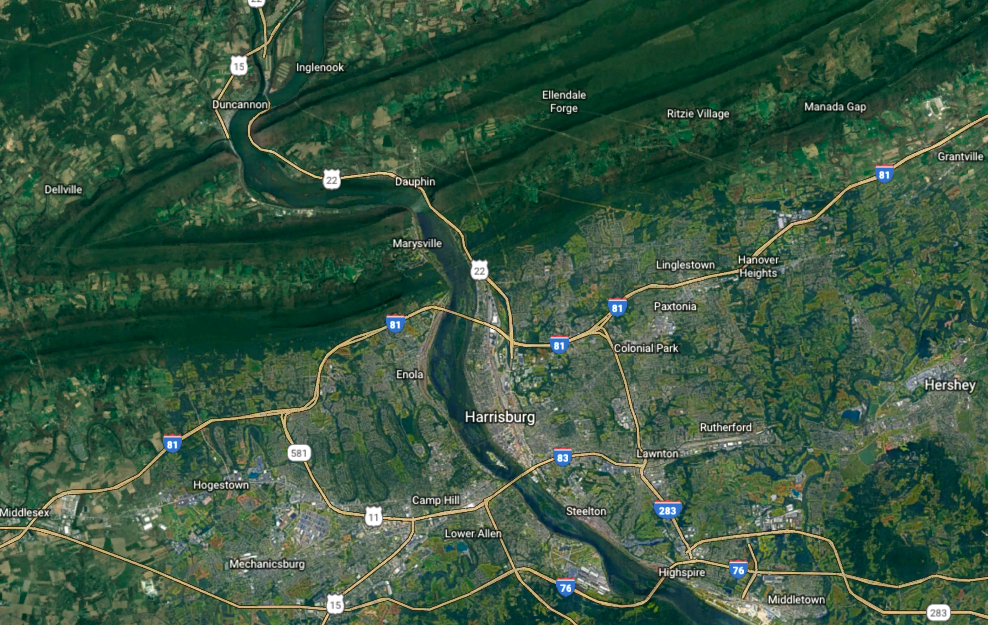
\includegraphics[width=3in]{figs/map}
\caption{Geographical map of Harrisburg showing the Susquehanna River running through the city and Appalachian Mountains to the north}
\label{map}
\end{figure}

% \subsection{Site information}

% This site collected the concentration of various pollutants including carbon monoxide (CO), sulfur dioxide (SO2) nitrogen dioxide (NO2) ozone (O3), fine particulate matter($PM_{10}$), and ultrafine particulate matter ($PM_{2.5}$) on an hourly basis between January 1, 2000 and December 31, 2016, except for the year of 2012, for which data was unavailable. Additionally, our analysis of the data revealed that different pollutants were measured for different ranges of time in the data we have available, likely as a result of changing measurement technologies, emissions standards, and equipment failure.

Based on the heavily industrialized history of Harrisburg and historical attainment information from the EPA, we selected $PM_{10}$ as the primary pollutant to focus our analysis on, with some analysis steps also using $PM_{2.5}$ data. Current major industrial sources of $PM_{10}$ and $PM_{2.5}$ that surround the monitoring site can be found in Table \ref{major_sources}. 


\begin{table*}[!t]
% increase table row spacing, adjust to taste
\renewcommand{\arraystretch}{1.3}
% if using array.sty, it might be a good idea to tweak the value of
% \extrarowheight as needed to properly center the text within the cells
\caption{Major $PM_{10}$ and $PM_{2.5}$ sources near site}
\label{major_sources}
\centering
% Some packages, such as MDW tools, offer better commands for making tables
% than the plain LaTeX2e tabular which is used here.
\begin{tabular}{|c|c|c|c|c|}
\hline

Source name &
Source Type &
% Location &
$PM_{10}$ (tons/yr) &
$PM_{2.5}$ (tons/yr) &
Distance from Site\\
\hline
STEELTON LLC &
Steel Plant &
% 215 S FRONT ST STEELTON PA  &
29 &
27 &
1.4 miles SSW\\

\hline

SUSQ RESOURCE MGMT COMPLEX &
Municipal Waste Combustor &
% 1670 S 19TH ST HARRISBURG PA  &
30 &
28 &
0.4 miles West\\

\hline

BRUNNER ISLAND &
Electricity Generation &
% 1400 WAGO RD YORK HAVEN PA &
1548 &
753 &
13 miles SW\\

\hline

NRG ENERGY CTR PAXTON &
Steam regional heating plant &
% 100 N 10TH ST HARRISBURG PA  &
6.43 &
6.41 &
2 miles NW\\

\hline
\end{tabular}
\end{table*}

% \subsection{Analysis process}
The data received by the air quality monitoring site was used to examine $PM_{10}$ levels from 2001 through 2011, the longest stretch of contiguous years with complete data. 
Having done so, we inspected the annual mean $PM_{10}$ levels for each year, as shown in Figure \ref{years}. In order to gain more visibility into specific sources of the particulate matter, we also analyzed diurnal concentration cycles, as computed by clustering measured data by hour of the day, then averaging through a specific year (Figure \ref{change_pm10}).

In order to further investigate specific sources of the measured pollutants, we augmented the data set with meteorological data from the nearby Capital City Airport, which is located a short distance southwest of our measurement site. In cases where wind data was unavailable for the exact time at which pollutant concentration data was taken, we linearly interpolated the nearest available wind vector measurements.

To inspect specific sources, we used Gaussian Dispersion Modelling to predict the concentration of pollutant we expect downwind from each site, based on prevailing winds and atmospheric stability (Figures \ref{windrose_1} and \ref{windrose_2}). We compare those predicted concentrations to observed concentrations, allowing us to analyze which specific pollutant sources likely contributed directly to the long-term trends seen earlier in the analysis.



\section{Results and Analysis}

\begin{figure}[!htbp]
\centering
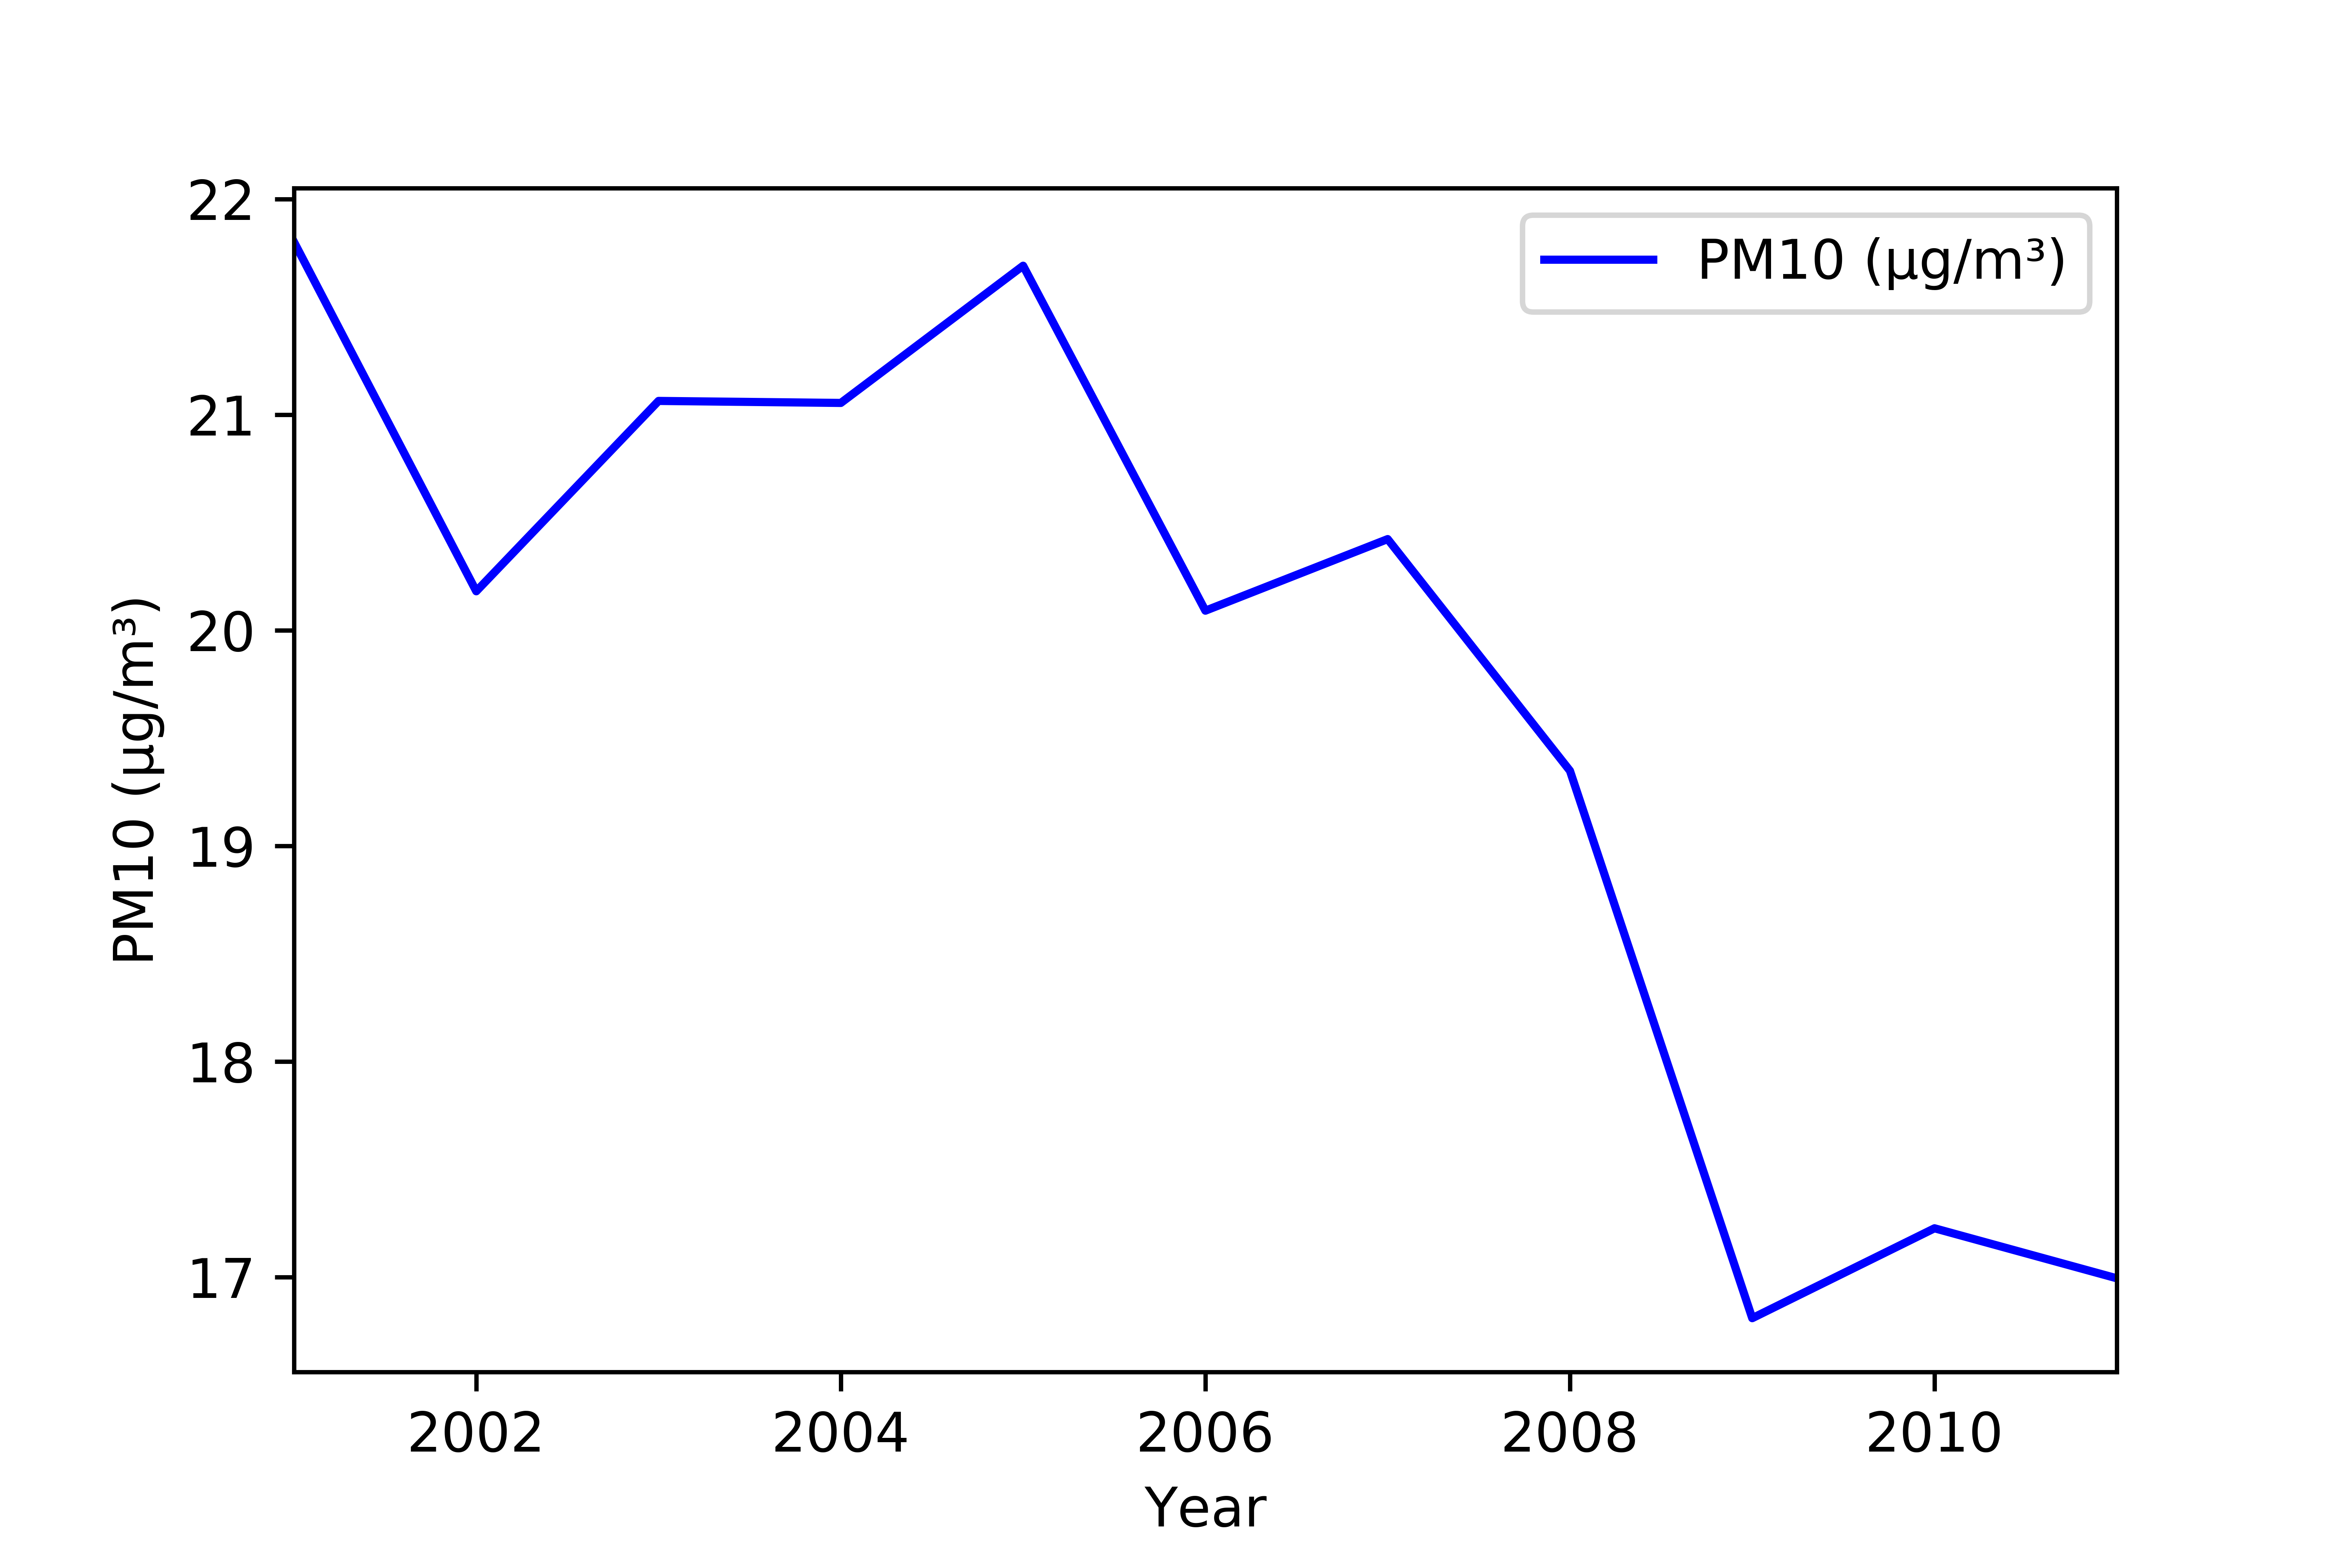
\includegraphics[width=2.5in]{figs/years}
\caption{Average annual concentration of $PM_{10}$, measured from 2001-2011}
\label{years}
\end{figure}

Using the largest continuous block of years of available $PM_{10}$ data (Jan 1 2001 - December 31 2011), Figure \ref{years} plots the mean annual $PM_{10}$ concentrations. It shows that $PM_{10}$ concentration in Harrisburg decreased during the duration of the study from $22 \frac{\mu g}{m^3}$ in 2001 to $17 \frac{\mu g}{m^3}$ in 2011, with the biggest decrease between 2008 and 2009.
An explanation behind this drastic change in emissions could be the change in politicians. Mayor Stephen Reed had been the mayor for 30 years, 1981 to mid-2009, and was arrested on corruption charges for not properly allocating or managing resources, misplacing audits, and conducting convoluted transactions, including swap agreements. 
This raises the question of whether or not pollution emissions from generators and factories in Harrisburg were adhering to regulations that correlate to the concentrations displayed in the graph, as will be discussed later in the analysis.


\begin{figure}[!htbp]
\centering
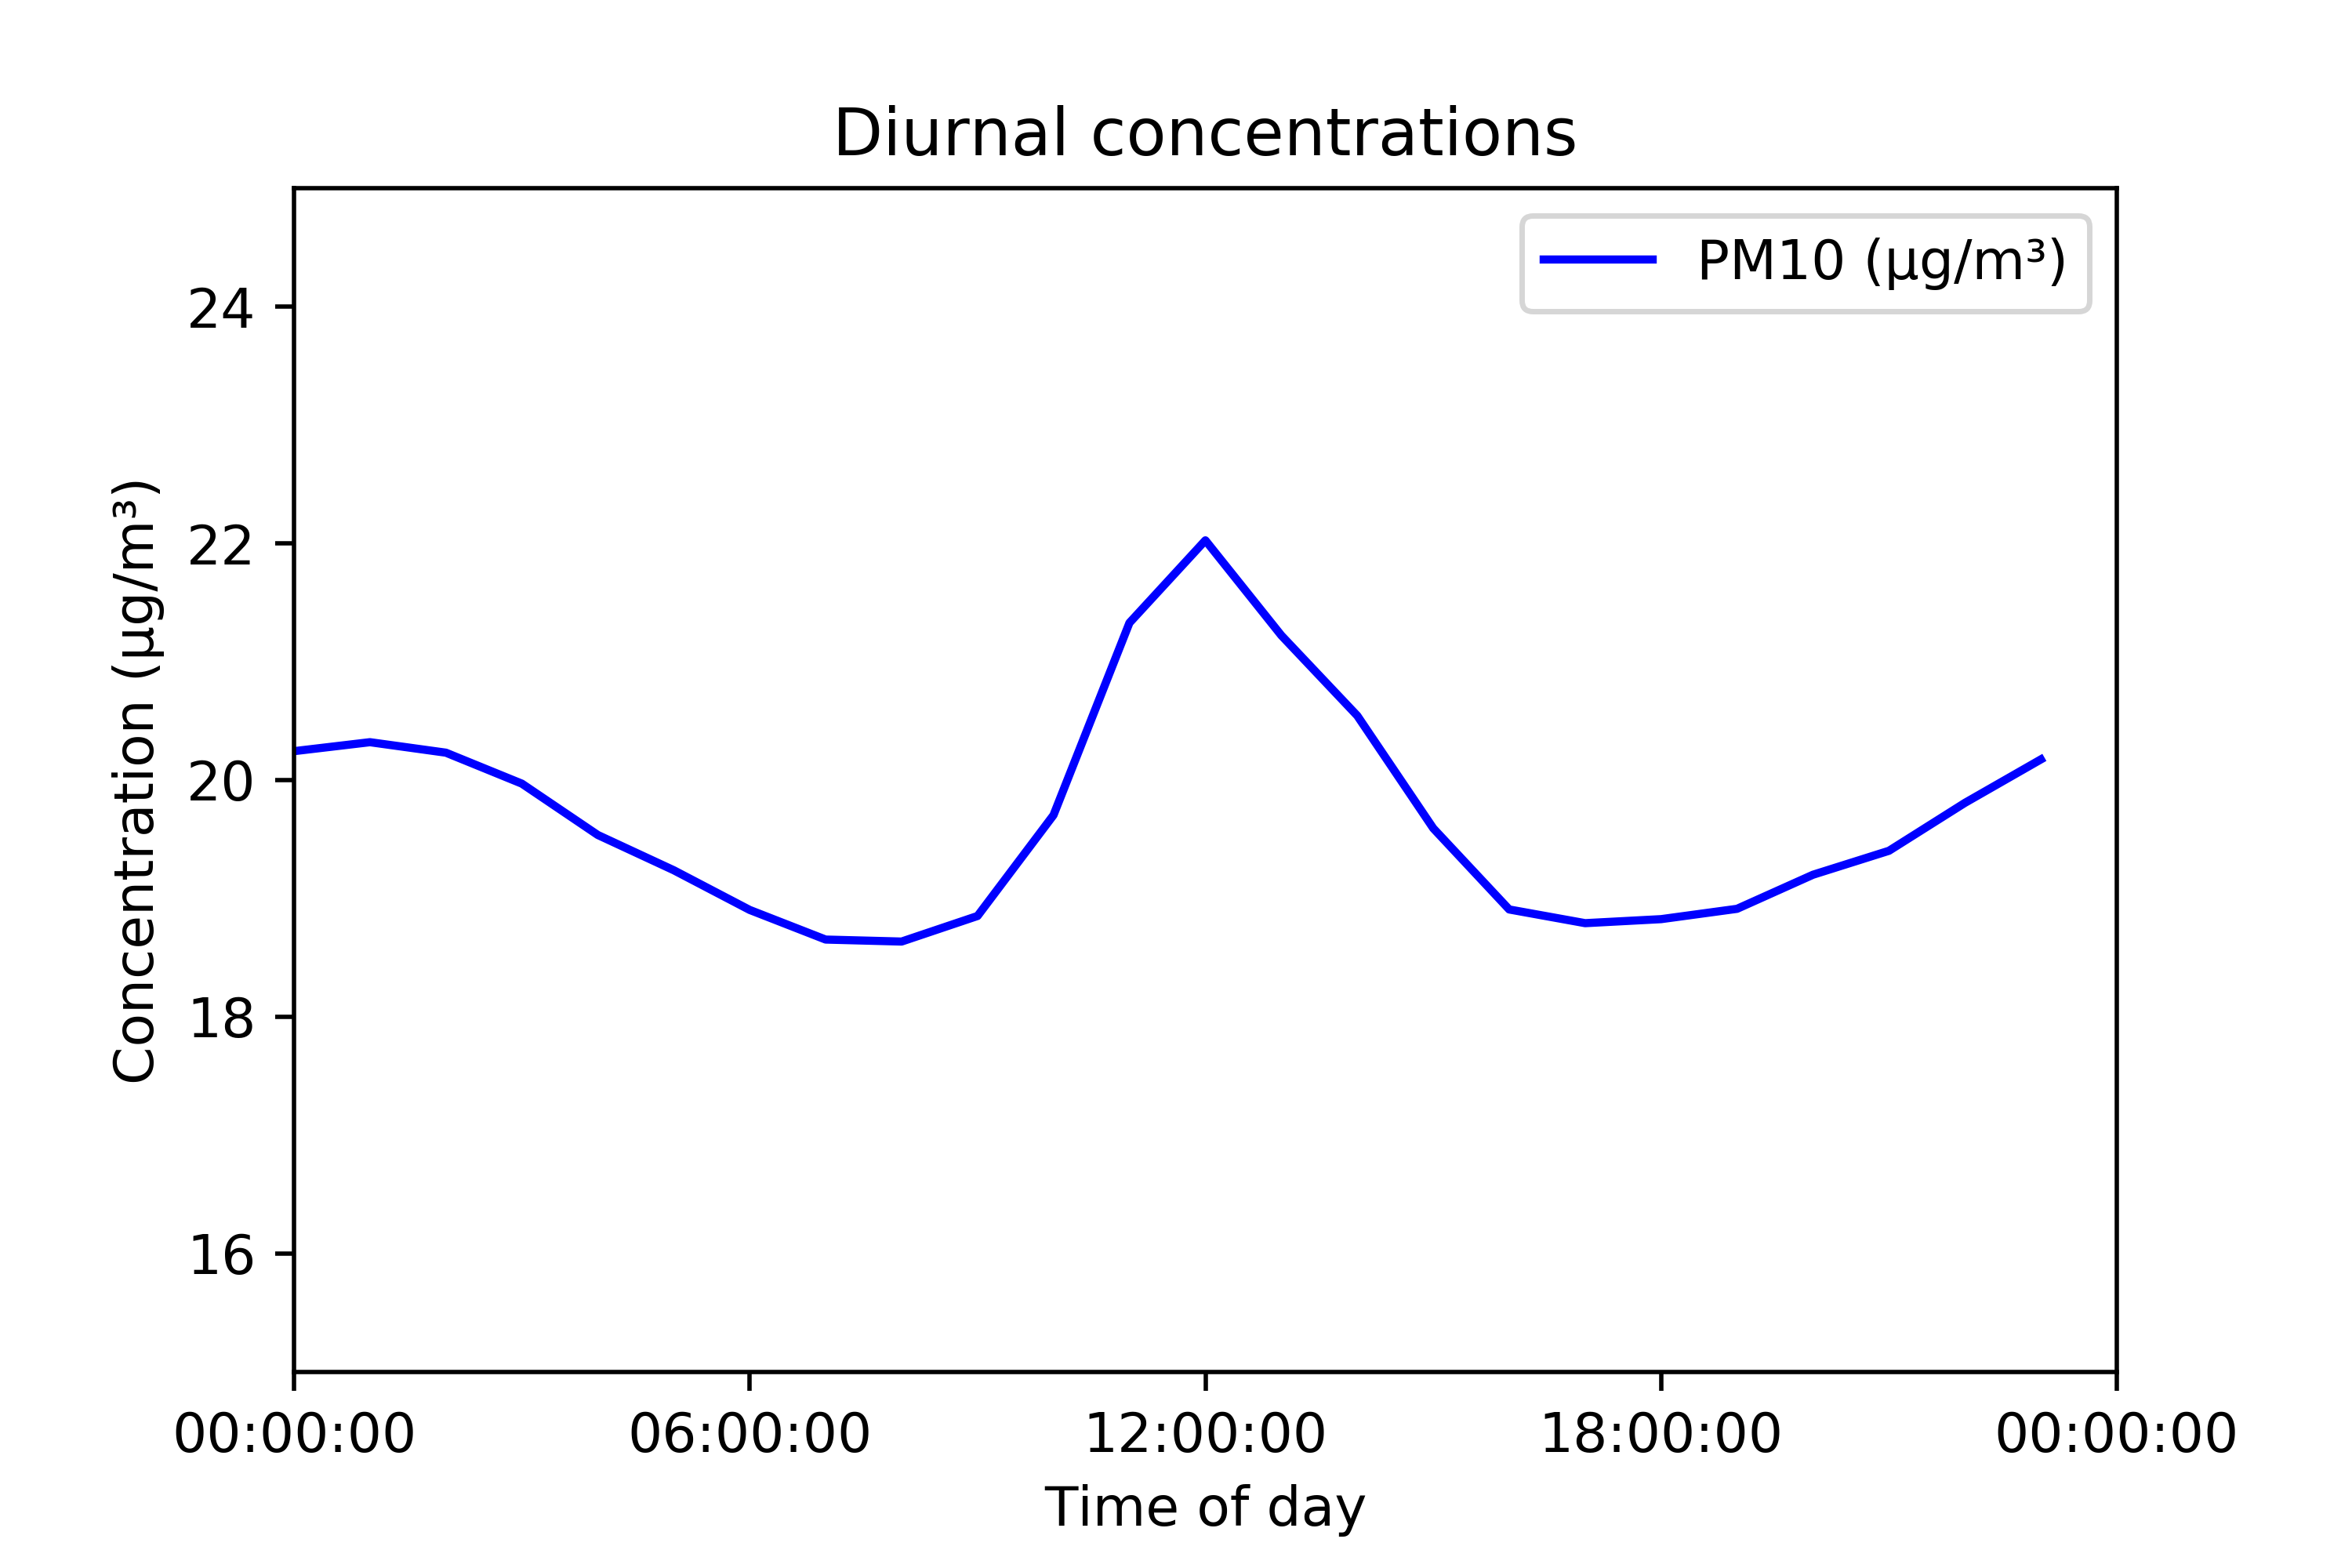
\includegraphics[width=3in]{figs/daily}
\caption{Diurnal cycle of $PM_{10}$ concentration, averaged over 2001-2011}
\label{daily}
\end{figure}


In order to further understand the character of $PM_{10}$ concentrations, we analyzed the diurnal cycle of $PM_{10}$ averaged over the entire data set. Figure \ref{daily} shows that $PM_{10}$ concentrations remain nearly steady at $19 \frac{\mu g}{m^3}$ for most of the day, with the notable exception of a sharp spike in concentrations beginning at 10:00am, peaking near $23 \frac{\mu g}{m^3}$ at noon.

Because this peak is so well-defined and consistent, we believe that it reflects a specific industrial source in conjunction with meteorological effects. As such, the most likely explanation for this peak is a single large particulate matter plume that is pushed towards the air monitoring site when the wind pattern shifts throughout the day. 


% \begin{figure}[!htbp]
% \centering
% 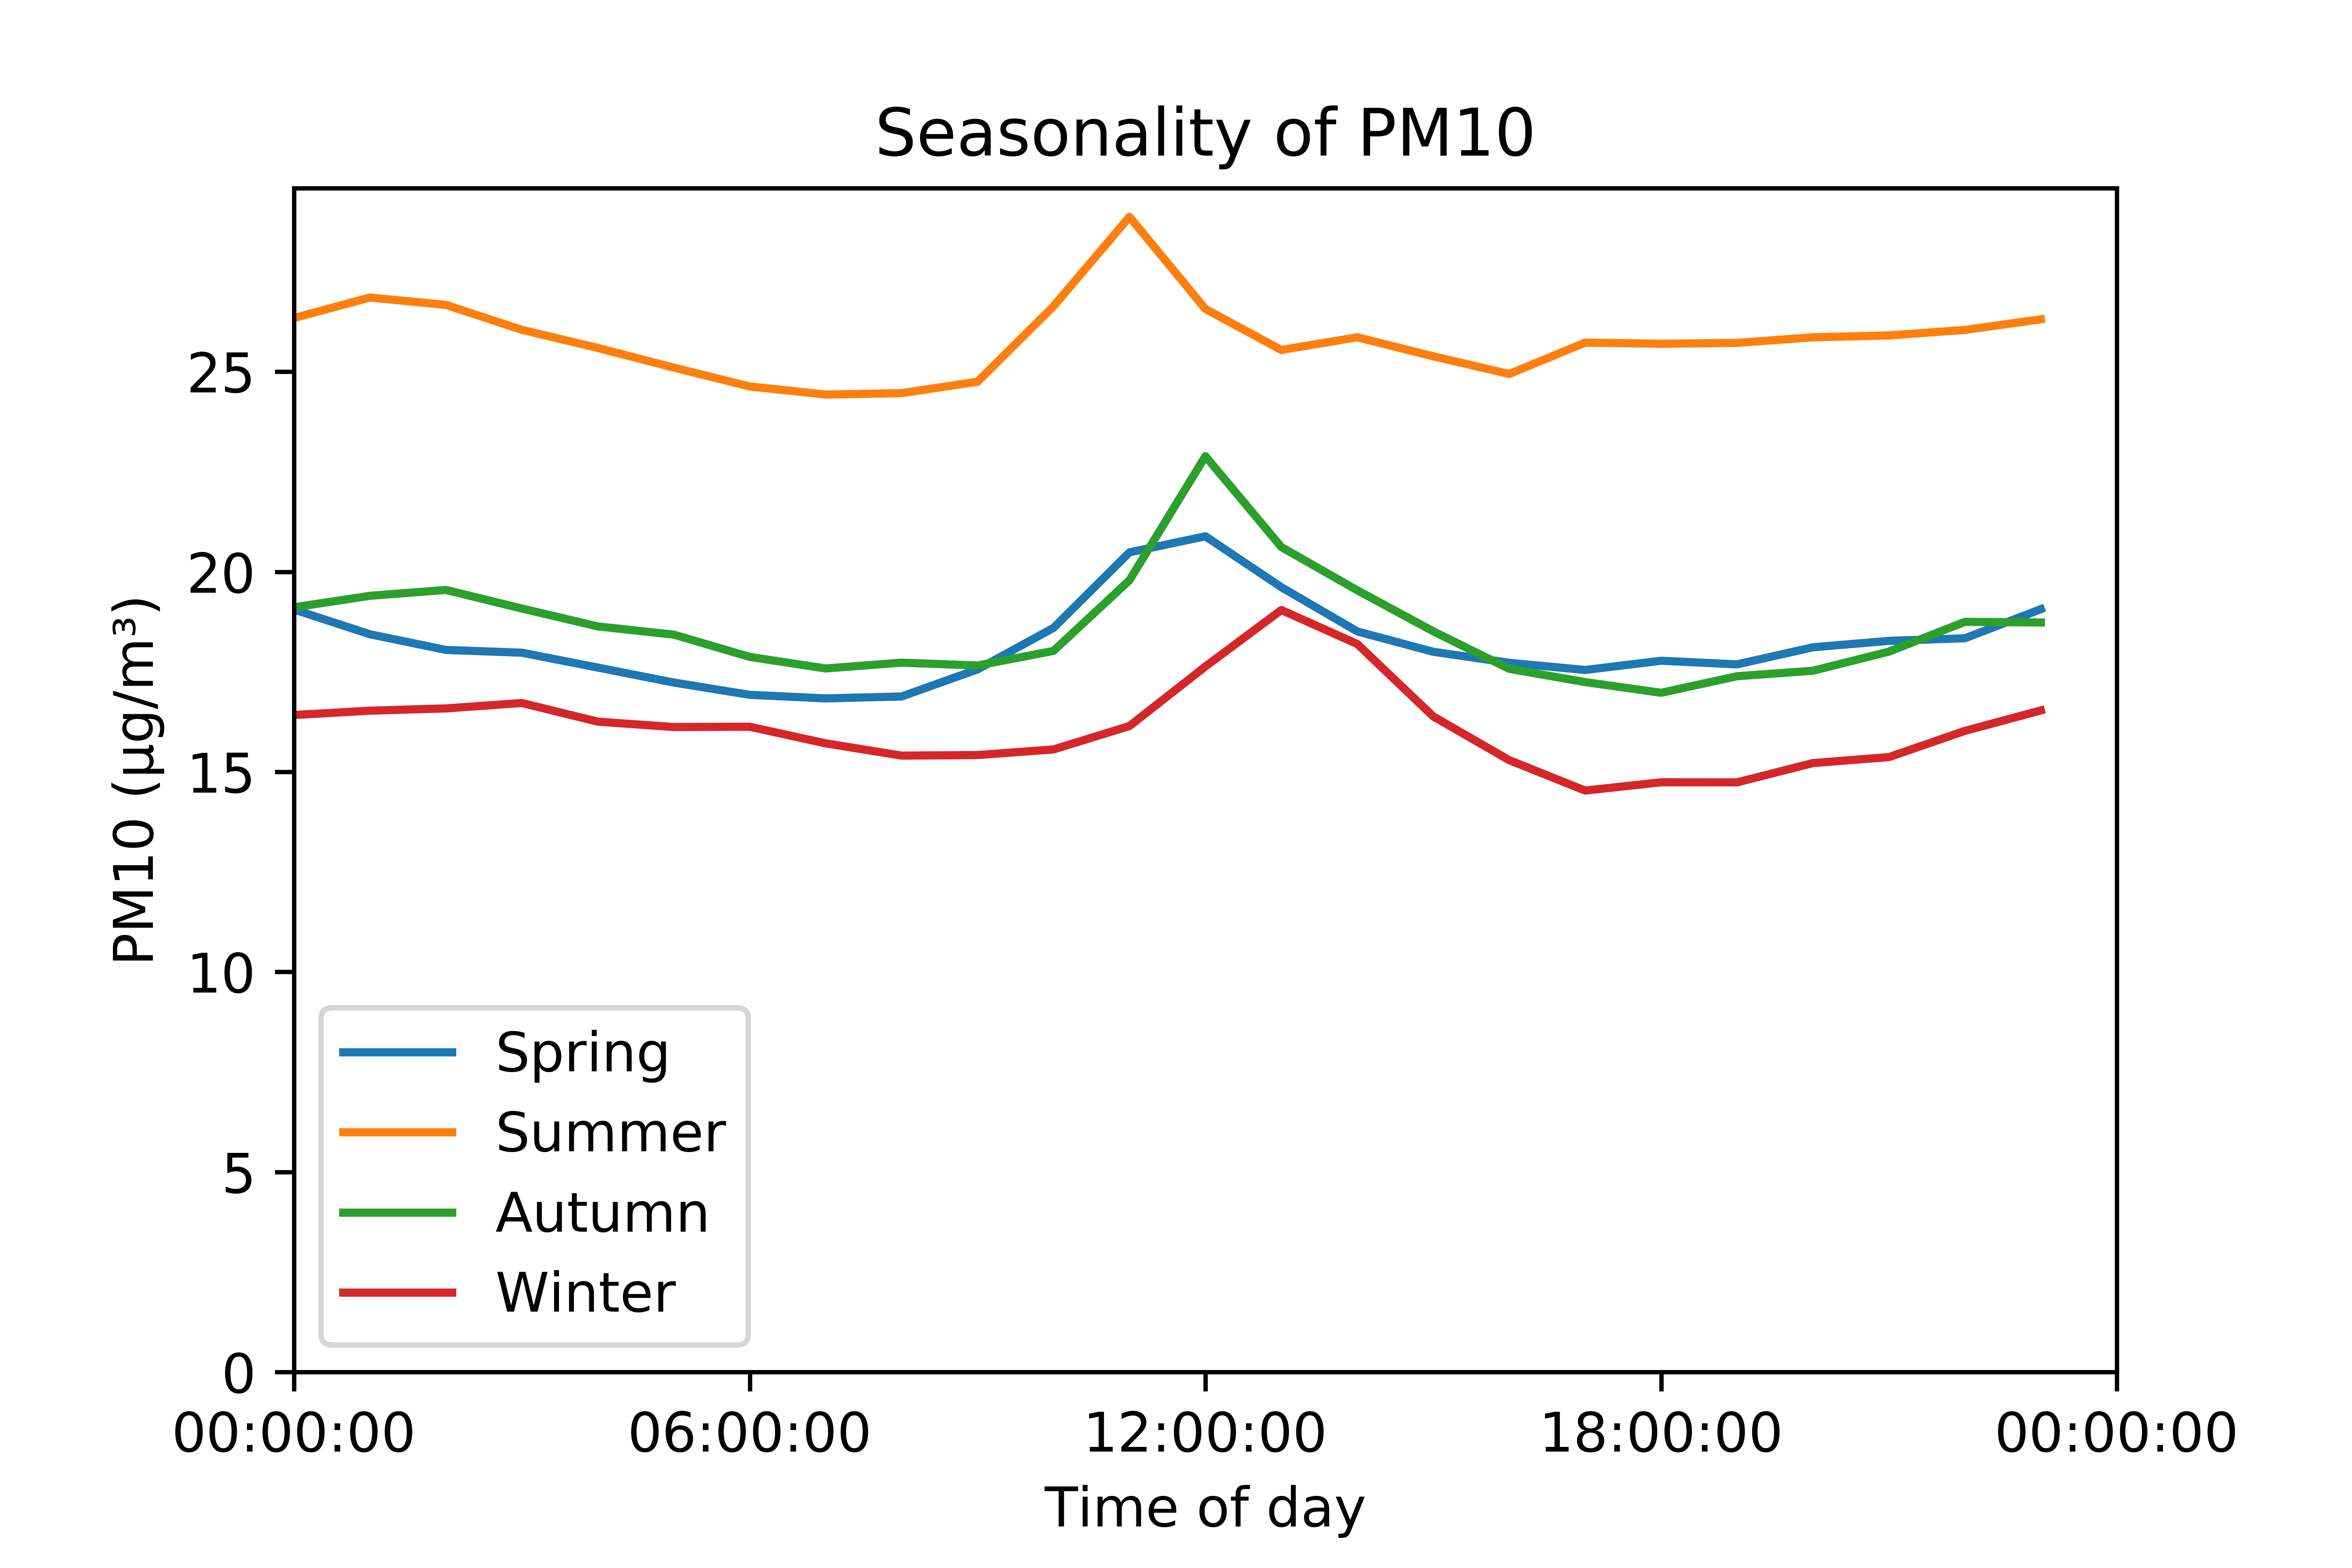
\includegraphics[width=3in]{figs/seasonality}
% \caption{Diurnal cycle of $PM_{10}$ concentration for each season}
% \label{seasonality}
% \end{figure}

% Further breaking down the the data from Figure \ref{daily}, Figure \ref{seasonality} shows the seasonality of $PM_{10}$ by averaging the measured quantities over the course of a day for each season, which shows that there is significant seasonal variation in overall levels of particulate matter, but the shape and magnitude of the 12:00 peak does not appear to vary significantly with the seasons. Additionally, the maximum of the peak occurs between 11:00 and 12:00 in all four seasons, although overall $PM_{10}$ levels are the lowest in the winter and highest in the summer.

% This implies that a natural origin of the sharp spike is unlikely, due to the four-season climate of Harrisburg\cite{normals}, and it is most likely the result of a single large industrial or commercial particulate source. In order to investigate the trends in the impact of this hypothesized source over time, we proceeded to analyze how the intensity of the spike in diurnal profiles has changed over the course of the study.

% It is unclear why concentrations are highest in summer, further research is needed in this area.


\begin{figure}[!htbp]
\centering
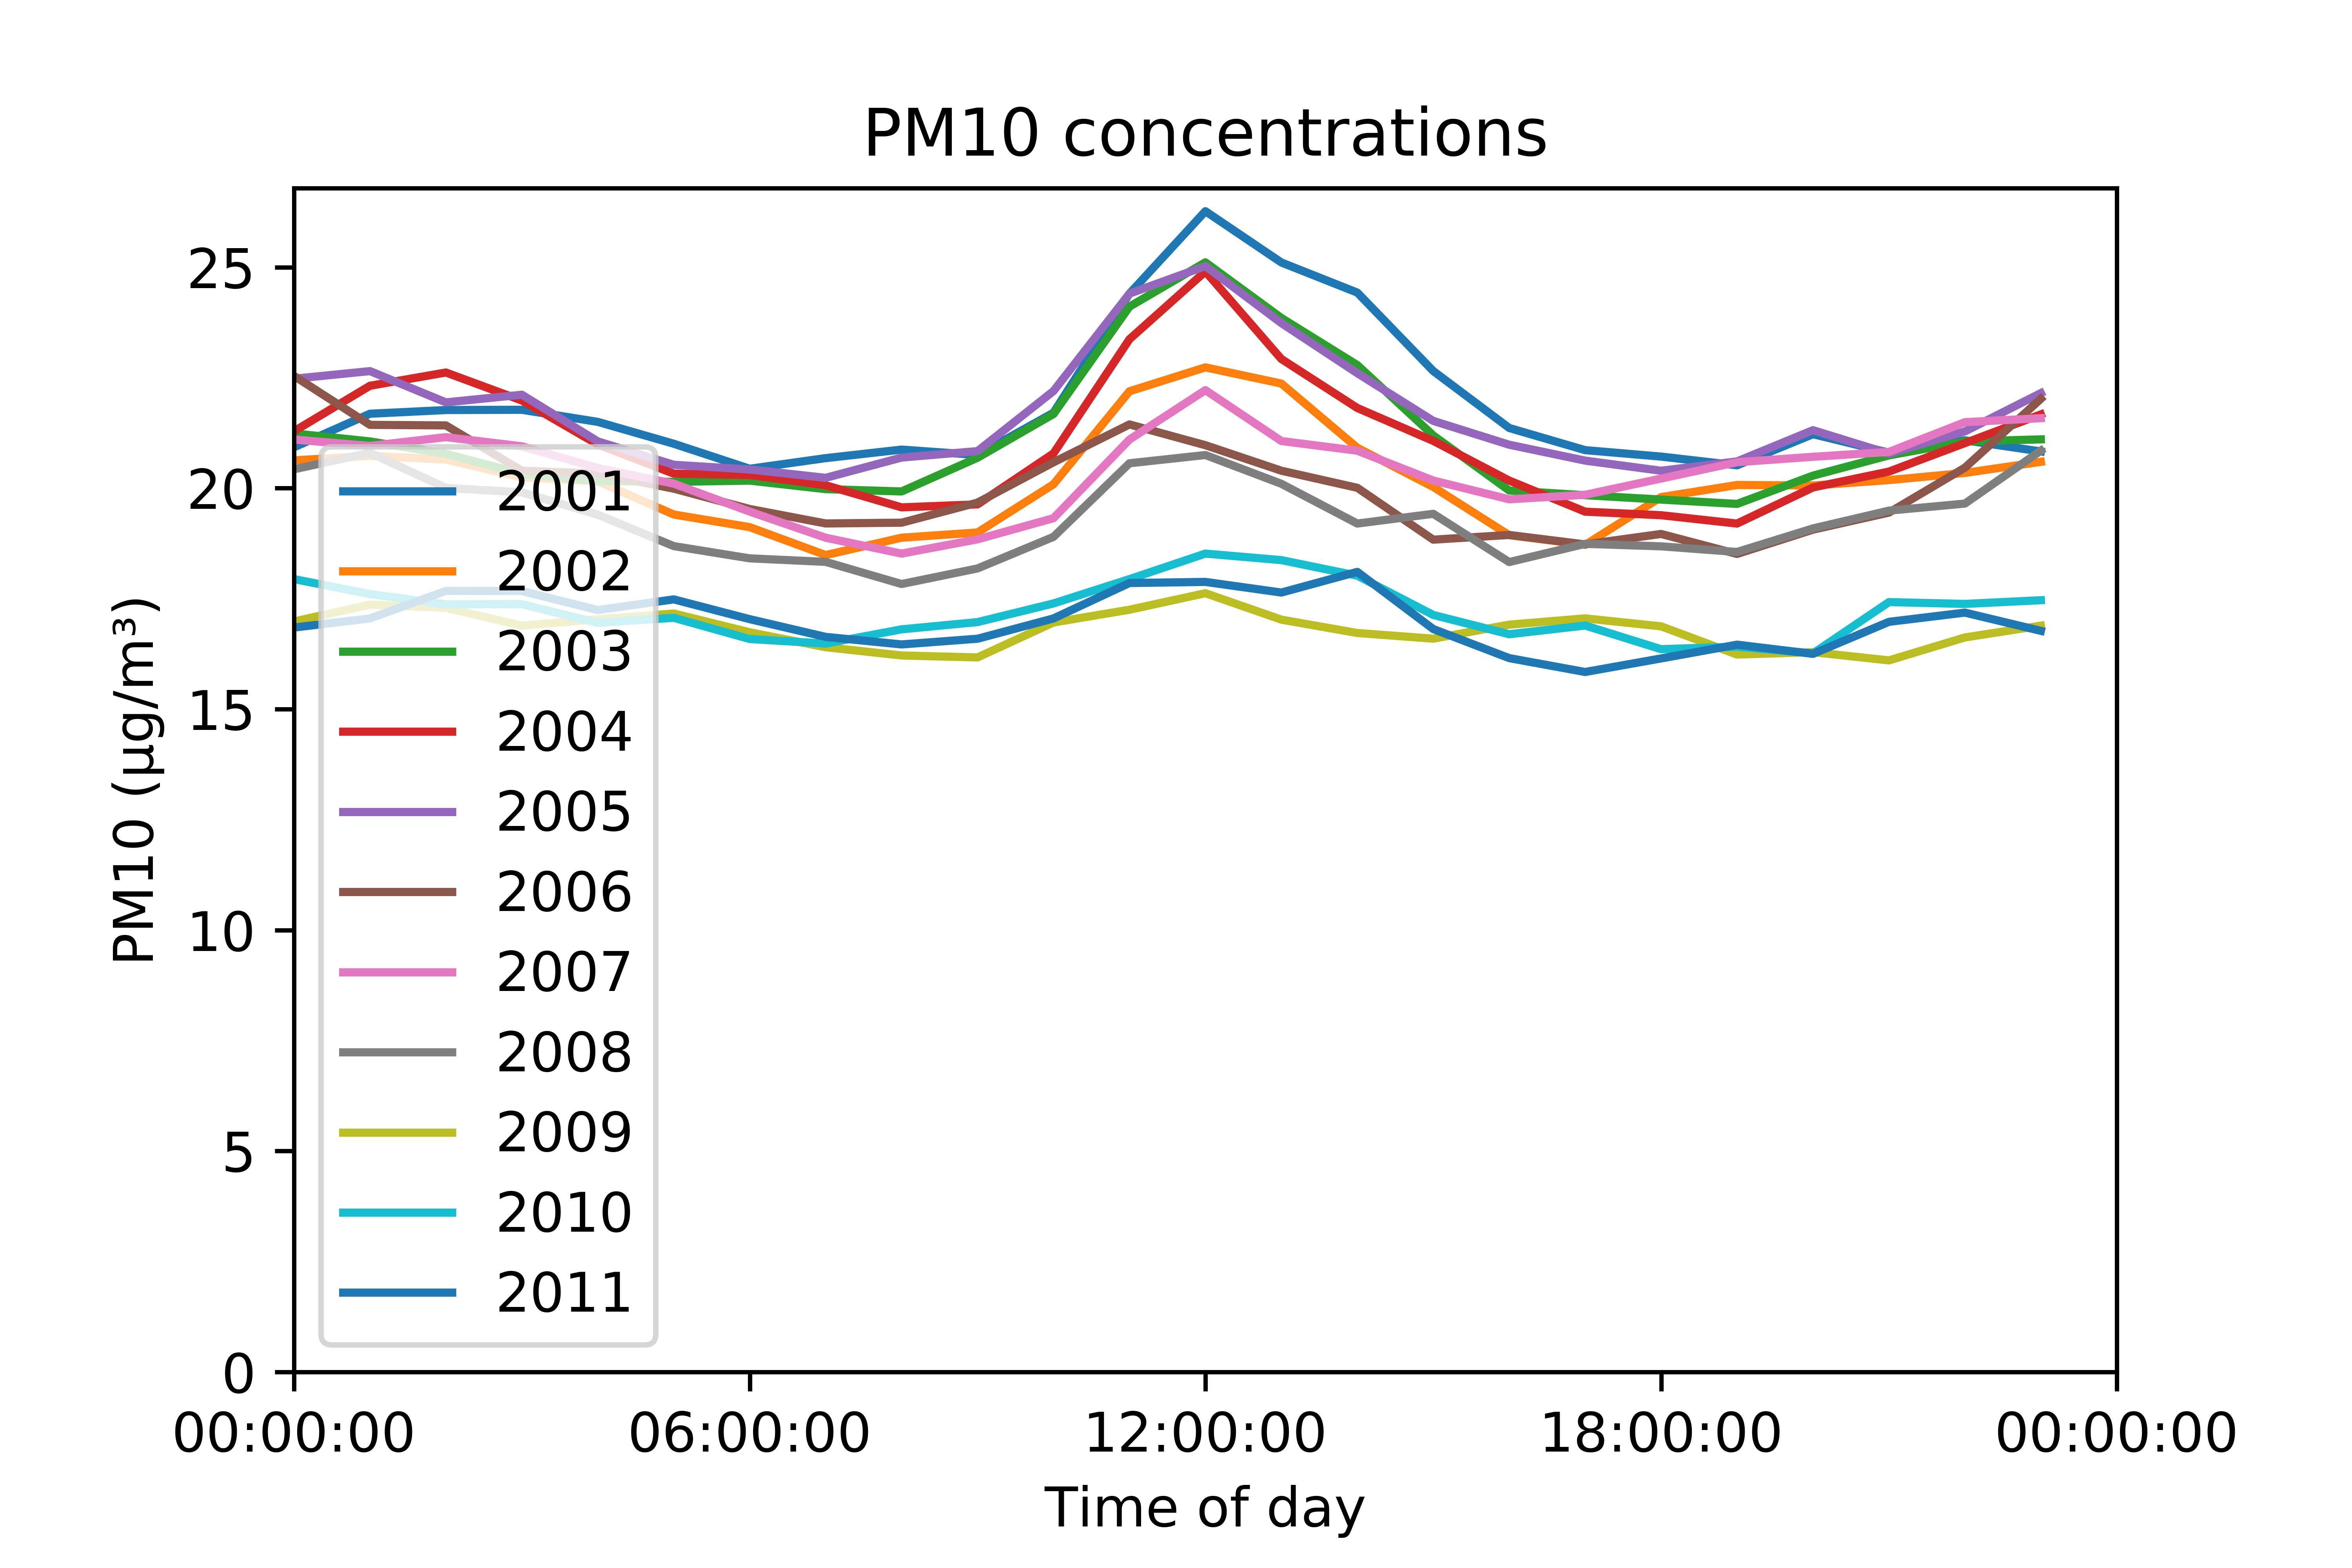
\includegraphics[width=3in]{figs/change_pm10}
\caption{Diurnal cycle of $PM_{10}$ concentration for each year between 2001 and 2011.}
\label{change_pm10}
\end{figure}

Figure \ref{change_pm10} displays the $PM_{10}$ measurements taken throughout a whole year averaged into a diurnal cycle. Each year is represented with its own curve spanning from 2001 to 2011. As expected from Figure \ref{years}, overall concentrations decrease during the duration of the study. Additionally, $PM_{10}$ concentrations peak at noon, in every year studied. However, in the earliest years of the study, the magnitude of that peak is more dramatic than that seen in Figure \ref{daily}, increasing by approximately 6 $\frac{\mu g}{m^3}$ between 9:00am and noon in 2001. In the later years of the study, the peak nearly disappears, representing an enhancement over the baseline of only 2 $\frac{\mu g}{m^3}$ during 2011. 

We hypothesize that this decrease in intensity of the midday peak, particularly in the period of 2006-2009, indicates the substantial decrease or effective emission regulations of a single large emissions point source, likely industrial in nature. Because prevailing wind direction changes during the course of the day for natural reasons, decreased emissions a large source near the measurement site could account for both the decrease in intensity of the peak, as well as some of the decrease in overall average levels. 

% \section{Work in progress}
% \begin{enumerate}
% \item
% Windrose plots for before and after the step-change noted above, attempting to isolate heading of large source

% \item
% Gaussian Dispersion modelling for Brunner Island coal plant and (possibly) Susquehanna Incinerator

% \end{enumerate}

In order to further investigate this source, we infused wind data from the Capital City Airport to understand the directions from which wind was blowing during times with high concentrations of $PM_{10}$. As seen in Figures \ref{windrose_1} and \ref{windrose_2}, the pollution concentrations are substantially higher when the wind is blowing straight from the west, averaging approximately $15 \frac{\mu g}{m^3}$. 

The concentrations from the West are substantially higher in the early years of the data (Figure \ref{windrose_1}), and decrease disproportionately by the later  years of the data (Figure \ref{windrose_2}). This leads us to believe that a significant proportion of the observed pollution levels decrease is due to reduction in $PM_{10}$ emitted straight to the west of the site. As indicated in Table \ref{major_sources}, the SRMC incinerator complex is a likely source of these pollutants, as we will investigate further below.

Additionally, Figures \ref{windrose_1} and \ref{windrose_2} indicate that winds from the south, although rare, also bring high $PM_{10}$ levels to the monitoring site, averaging approximately $22 \frac{\mu g}{m^3}$. The most likely source of these pollutant concentrations is the Brunner Island coal power plant. 

% Renderings of these two facilities are included in Figure \ref{renderings}.

\begin{figure}[!htbp]
\centering
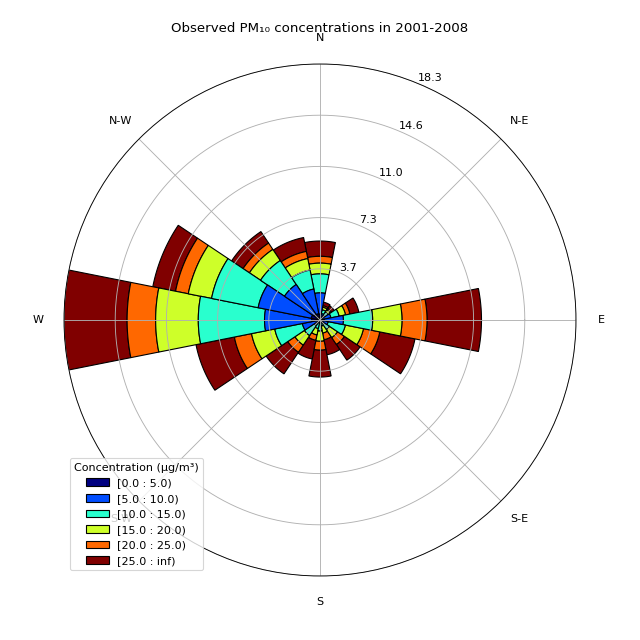
\includegraphics[width=3in]{figs/windrose_2}
\caption{Pollution levels as a function of prevailing wind speeds, between 2001 and 2008. Notice the substantially higher pollution concentrations when the wind is coming from the West, Southwest, and South, compared to the Northwest and North.}
\label{windrose_1}
\end{figure}

\begin{figure}[!htbp]
\centering
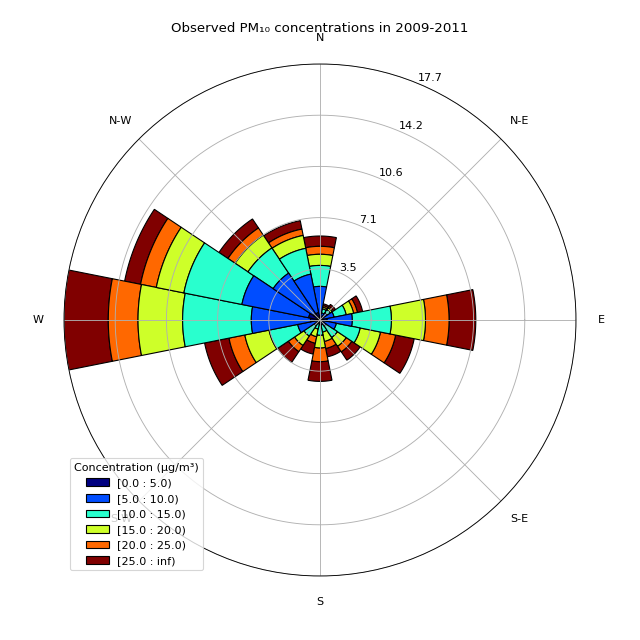
\includegraphics[width=3in]{figs/windrose_3}
\caption{Pollution levels as a function of prevailing wind speeds, between 2009 and 2011. Notice the overall decrease in concentrations, as well as the significant drop in high-concentrations from the west.}
\label{windrose_2}
\end{figure}

% \begin{figure}[!htbp]
% \centering
% 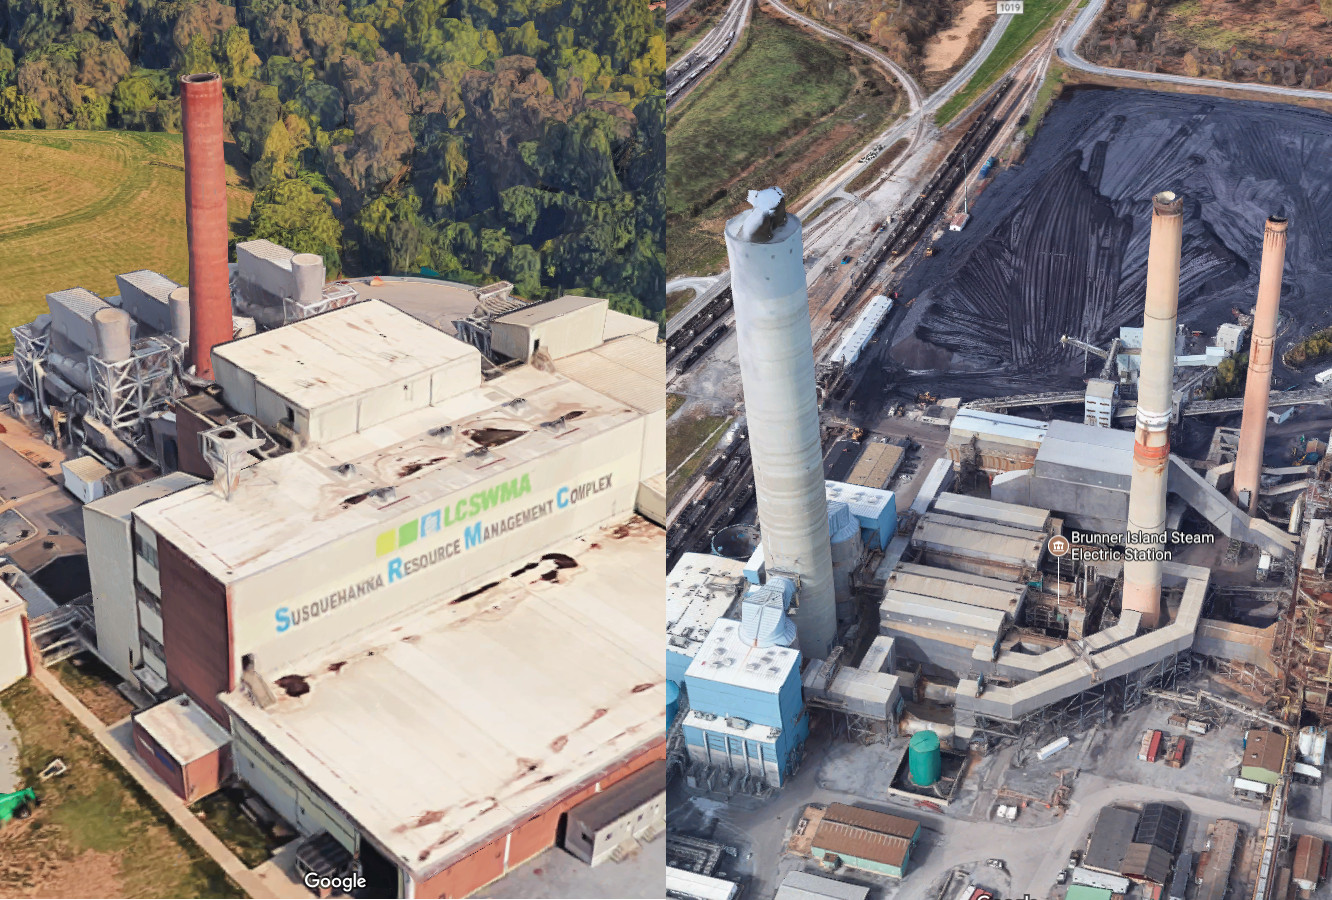
\includegraphics[width=3in]{figs/renderings.jpg}
% \caption{Renderings of the Susquehanna Resource Management Complex on the left and the Brunner Island coal power plant on the right. Data acquired through Google Maps.}
% \label{renderings}
% \end{figure}

To understand the contribution of these sources to the measured pollution concentrations at the site, we conducted a Gaussian dispersion analysis using point source emission data from Table \ref{major_sources} and wind speed data averaged over all measurements with the given source direction. Figure \ref{incinerator} shows the resulting plume shape from the incinerator on a day with stability class C, typical of a summer day in the Harrisburg area. Maximum concentrations at the site reach $12 \frac{\mu g}{m^3}$, very close to the $15 \frac{\mu g}{m^3}$ measured in air from the west. This indicates that $PM_{10}$ emissions from the incinerator site likely comprise a significant fraction of the ground-level pollutant concentration observed when wind is coming from the west.

\begin{figure}[htbp]
\centering
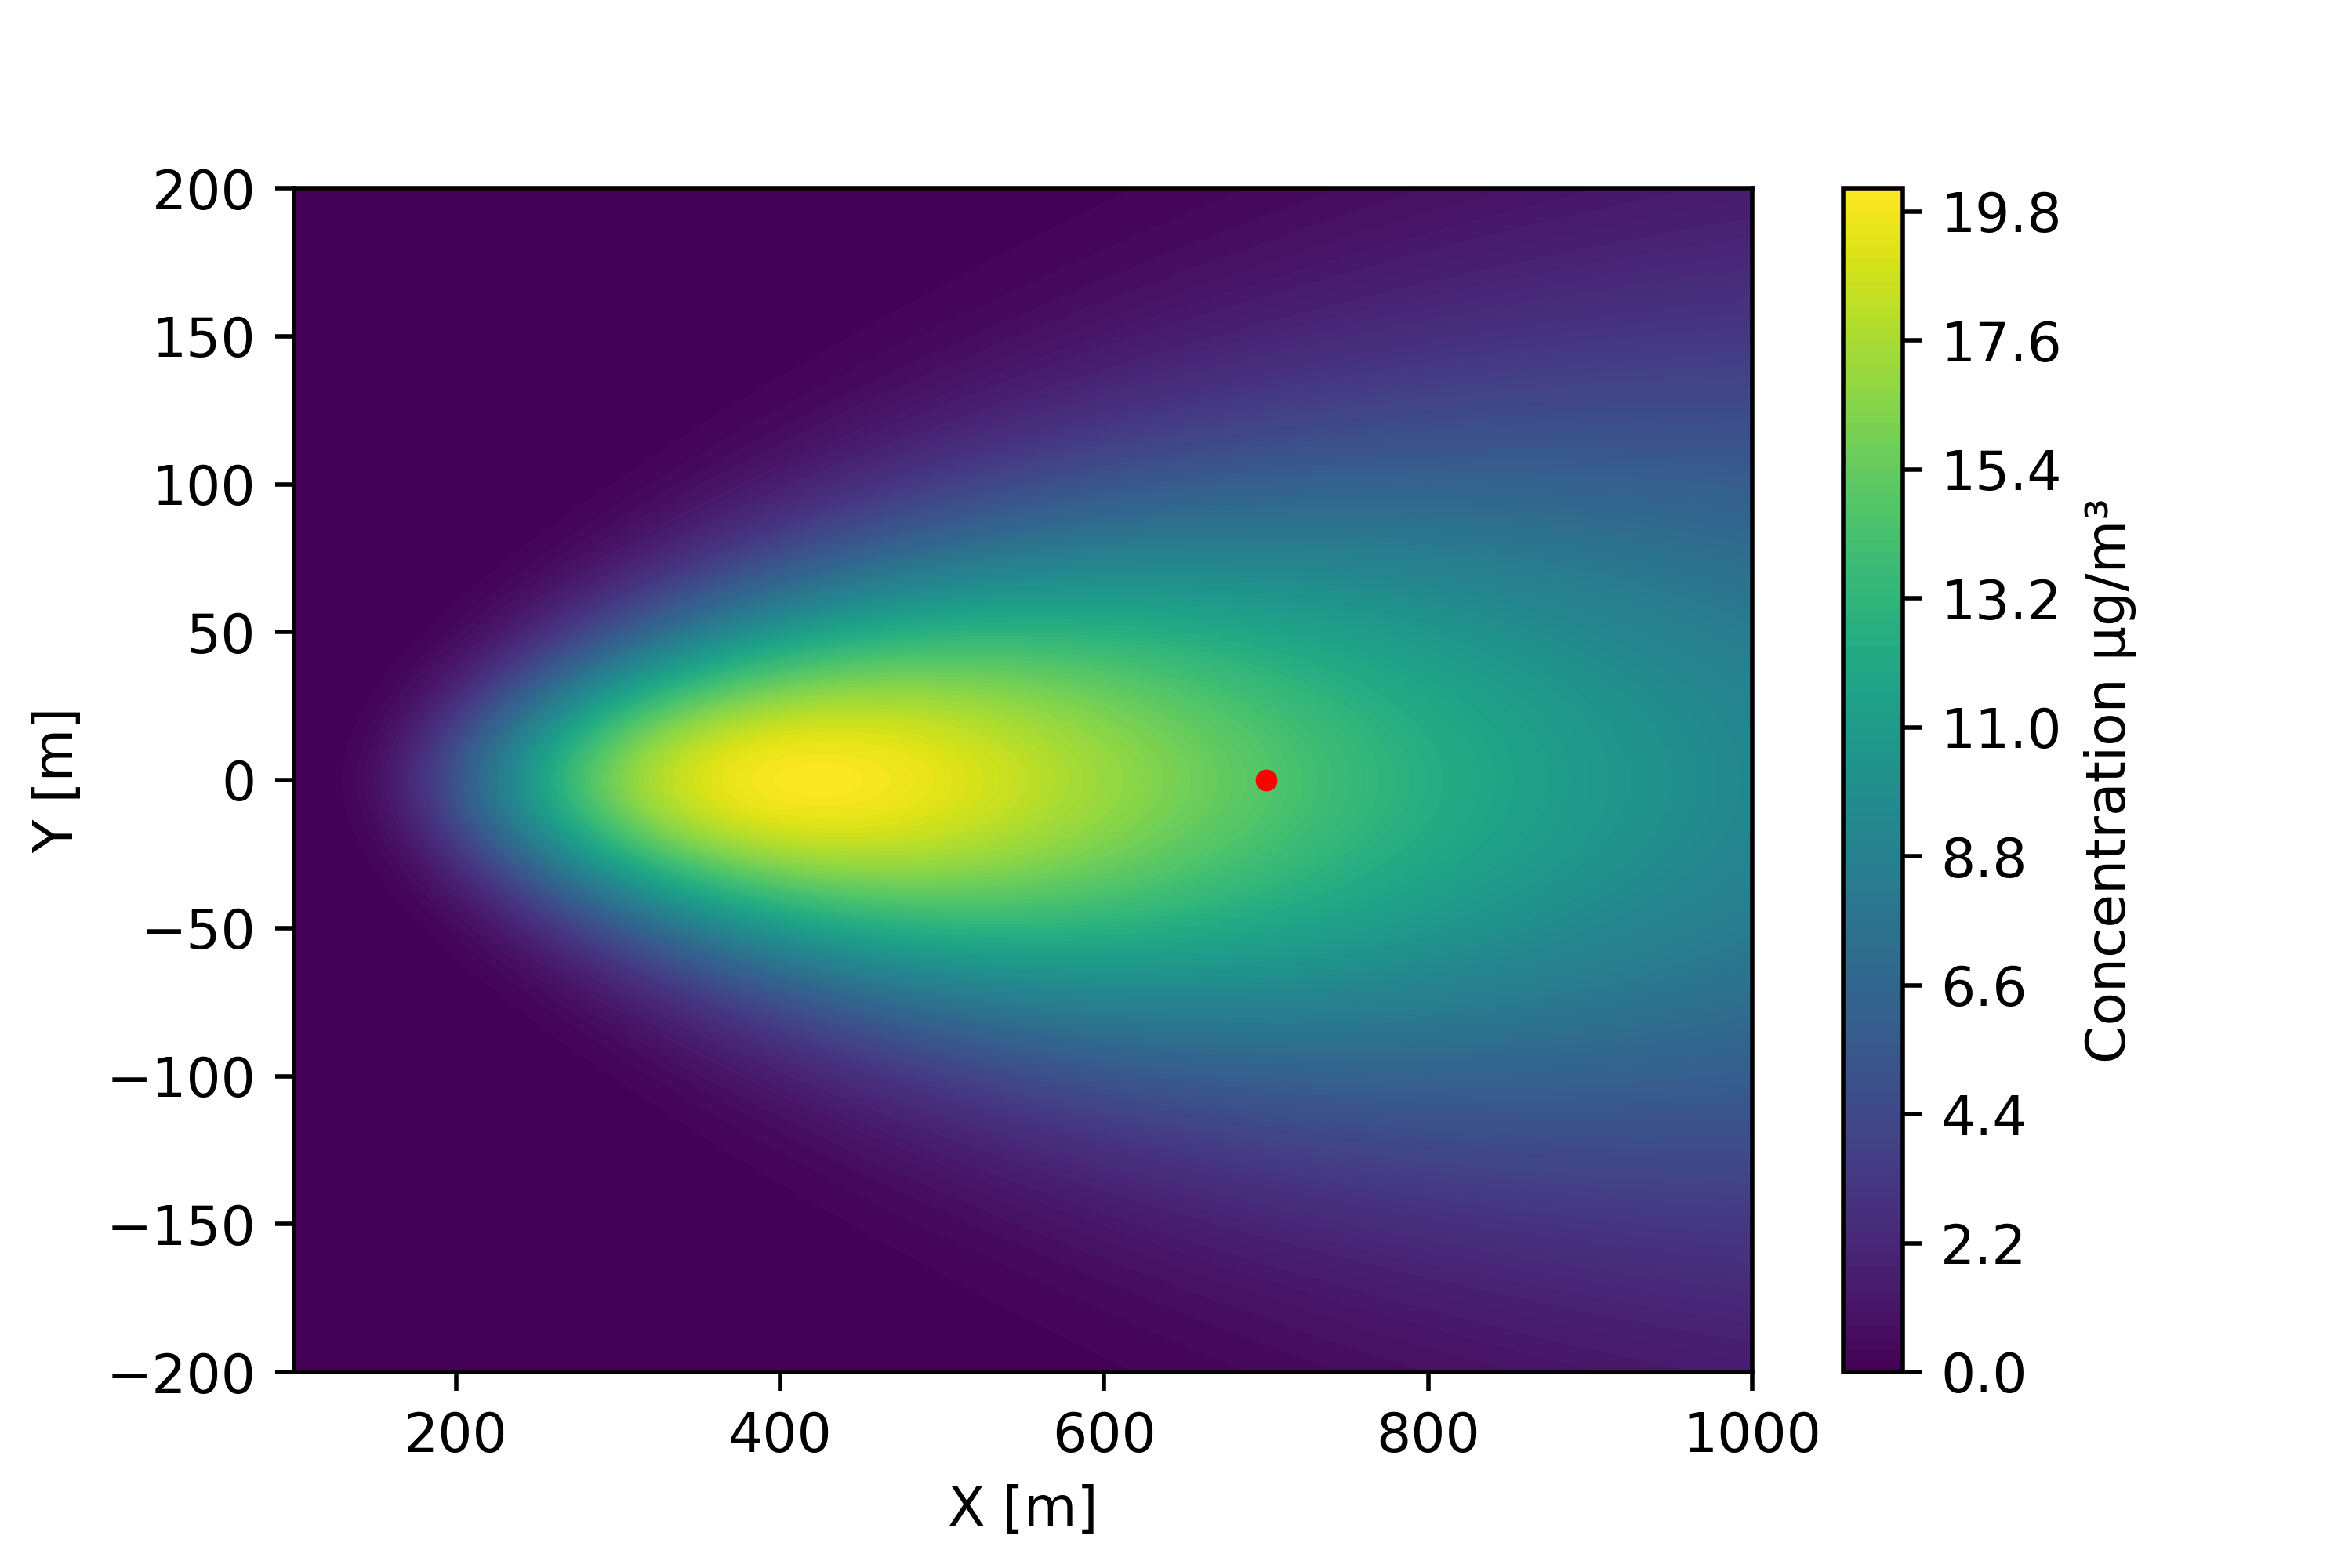
\includegraphics[width=3in]{figs/incinerator_cloud}
\caption{Gaussian dispersion model of particulate distribution from SRMC incinerator. The red dot indicates the distance of the measurement site.}
\label{incinerator}
\end{figure}

Similarly, Figure \ref{powerplant} shows the dispersion plume from the Brunner Island coal power plant with a typical wind blowing north and class C stability. This model indicates that peak concentrations at the measurement site should be $18 \frac{\mu g}{m^3}$, which represents a substantial fraction of the $22 \frac{\mu g}{m^3}$ observed in available data. This indicates that the Brunner Island power plant, even though it is located several miles outside of Harrisburg, can still account for a significant fraction of the pollution in the city on days with particularly unlucky meteorological conditions.

\begin{figure}[htbp]
\centering
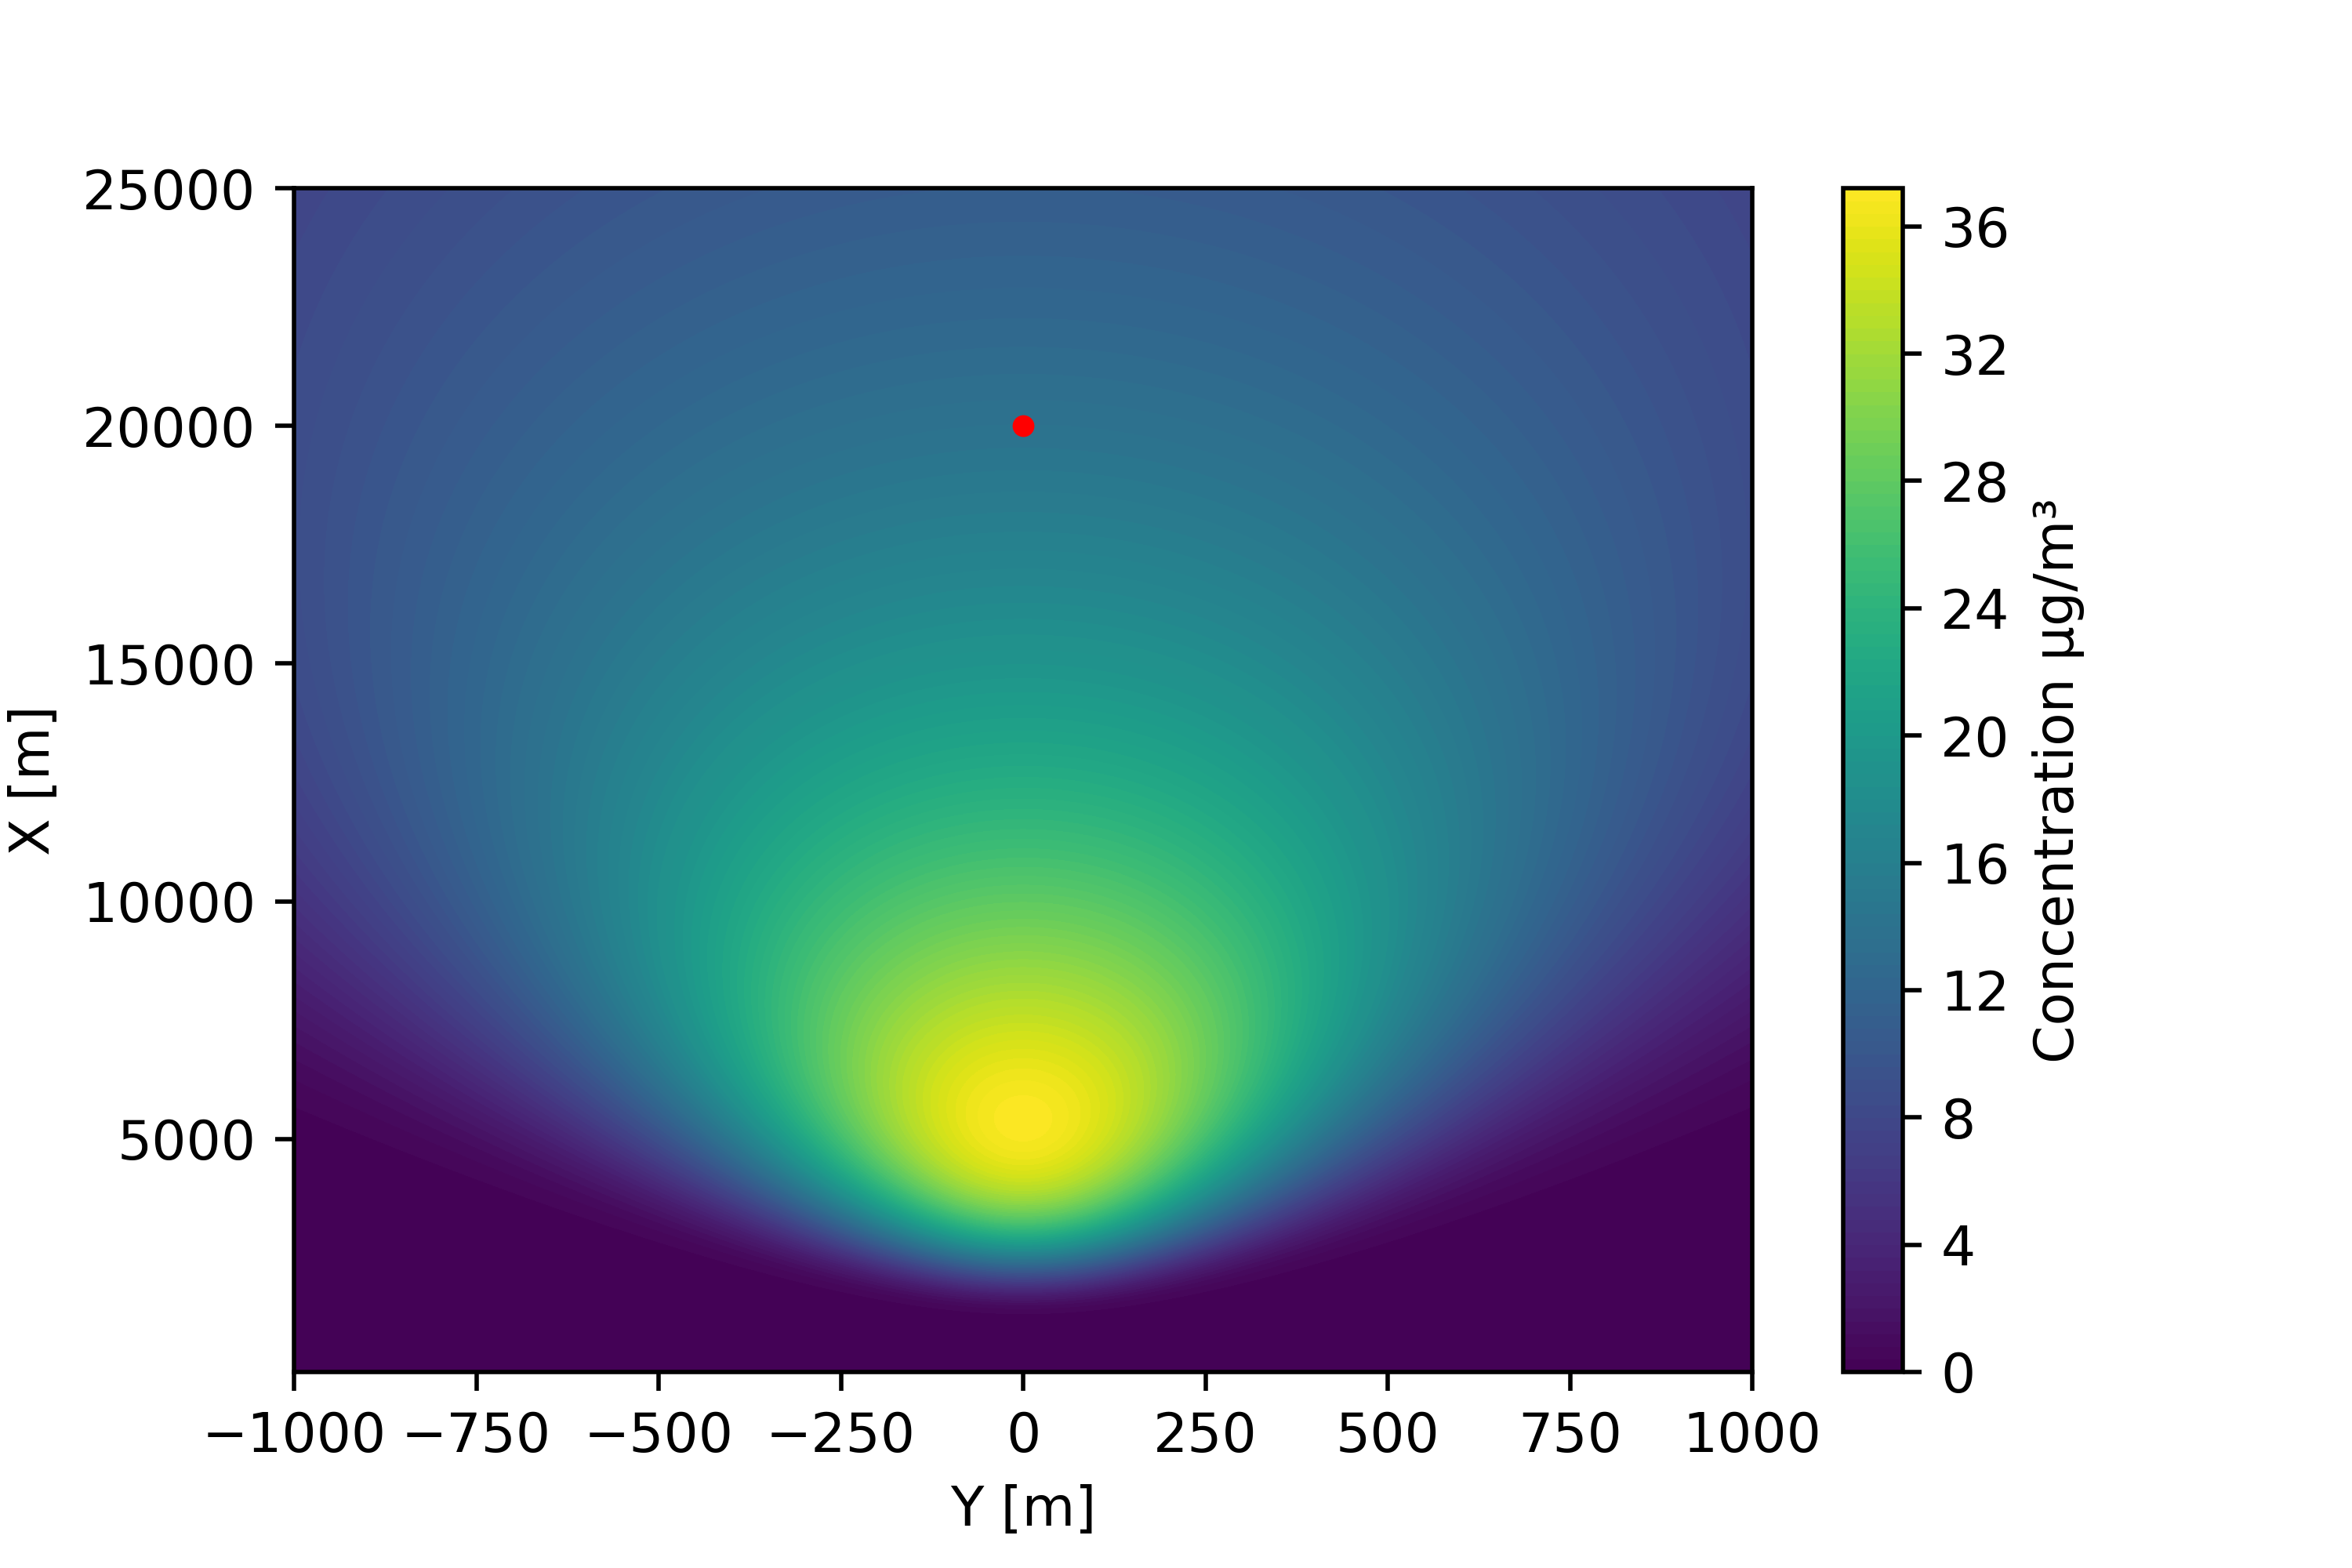
\includegraphics[width=3in]{figs/coal_cloud}
\caption{Gaussian dispersion model of particulate distribution from the Brunner Island coal power plant. The red dot indicates the distance of the measurement site.}
\label{powerplant}
\end{figure}


% An example of a floating figure using the graphicx package.
% Note that \label must occur AFTER (or within) \caption.
% For figures, \caption should occur after the \includegraphics.
% Note that IEEEtran v1.7 and later has special internal code that
% is designed to preserve the operation of \label within \caption
% even when the captionsoff option is in effect. However, because
% of issues like this, it may be the safest practice to put all your
% \label just after \caption rather than within \caption{}.
%
% Reminder: the "draftcls" or "draftclsnofoot", not "draft", class
% option should be used if it is desired that the figures are to be
% displayed while in draft mode.
%
% \begin{figure}[!t]
% \centering
% 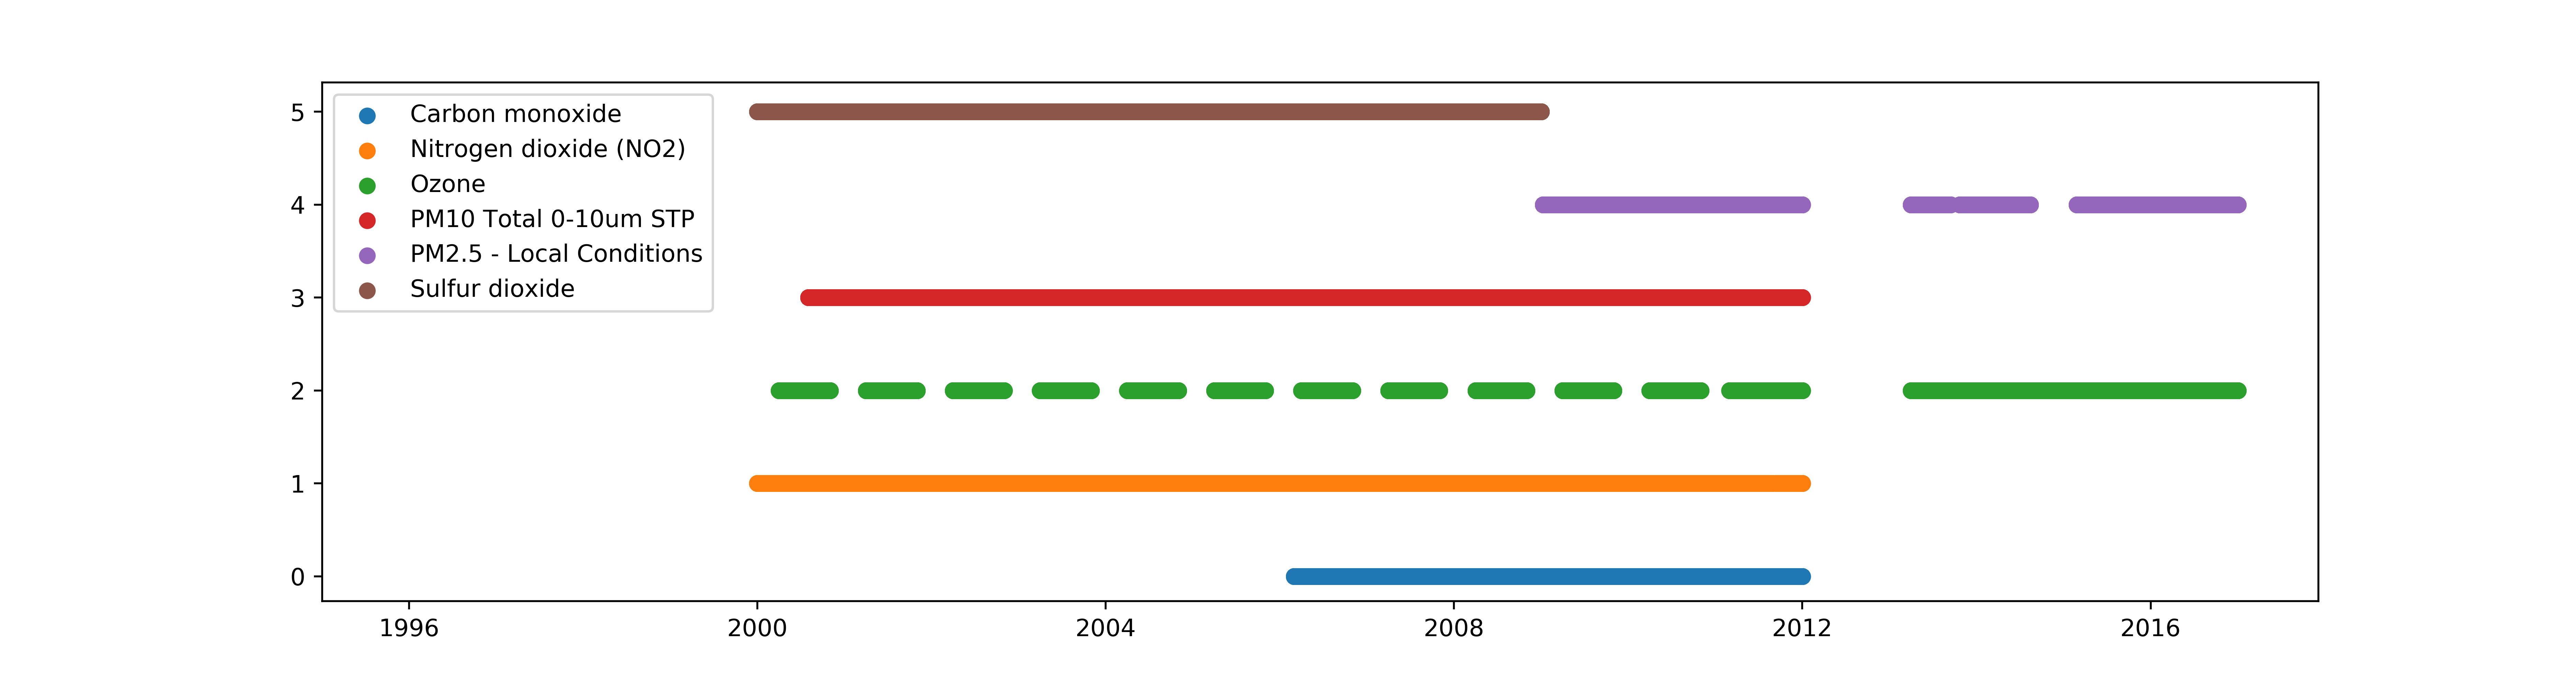
\includegraphics[width=8in]{figs/data_availability.png}
% % via \DeclareGraphicsExtensions.
% \caption{Availability of measurement data for various pollutants}
% \label{data_availability}
% \end{figure}

% Note that IEEE typically puts floats only at the top, even when this
% results in a large percentage of a column being occupied by floats.





% \section{Conclusion}
% Data analysis of air pollutant measurements from Harrisburg, PA indicates that two major sources contribute to 



% \begin{figure}[htbp]
% % TODO: figure out how to make this figure large and across the whole page
% \centering
% 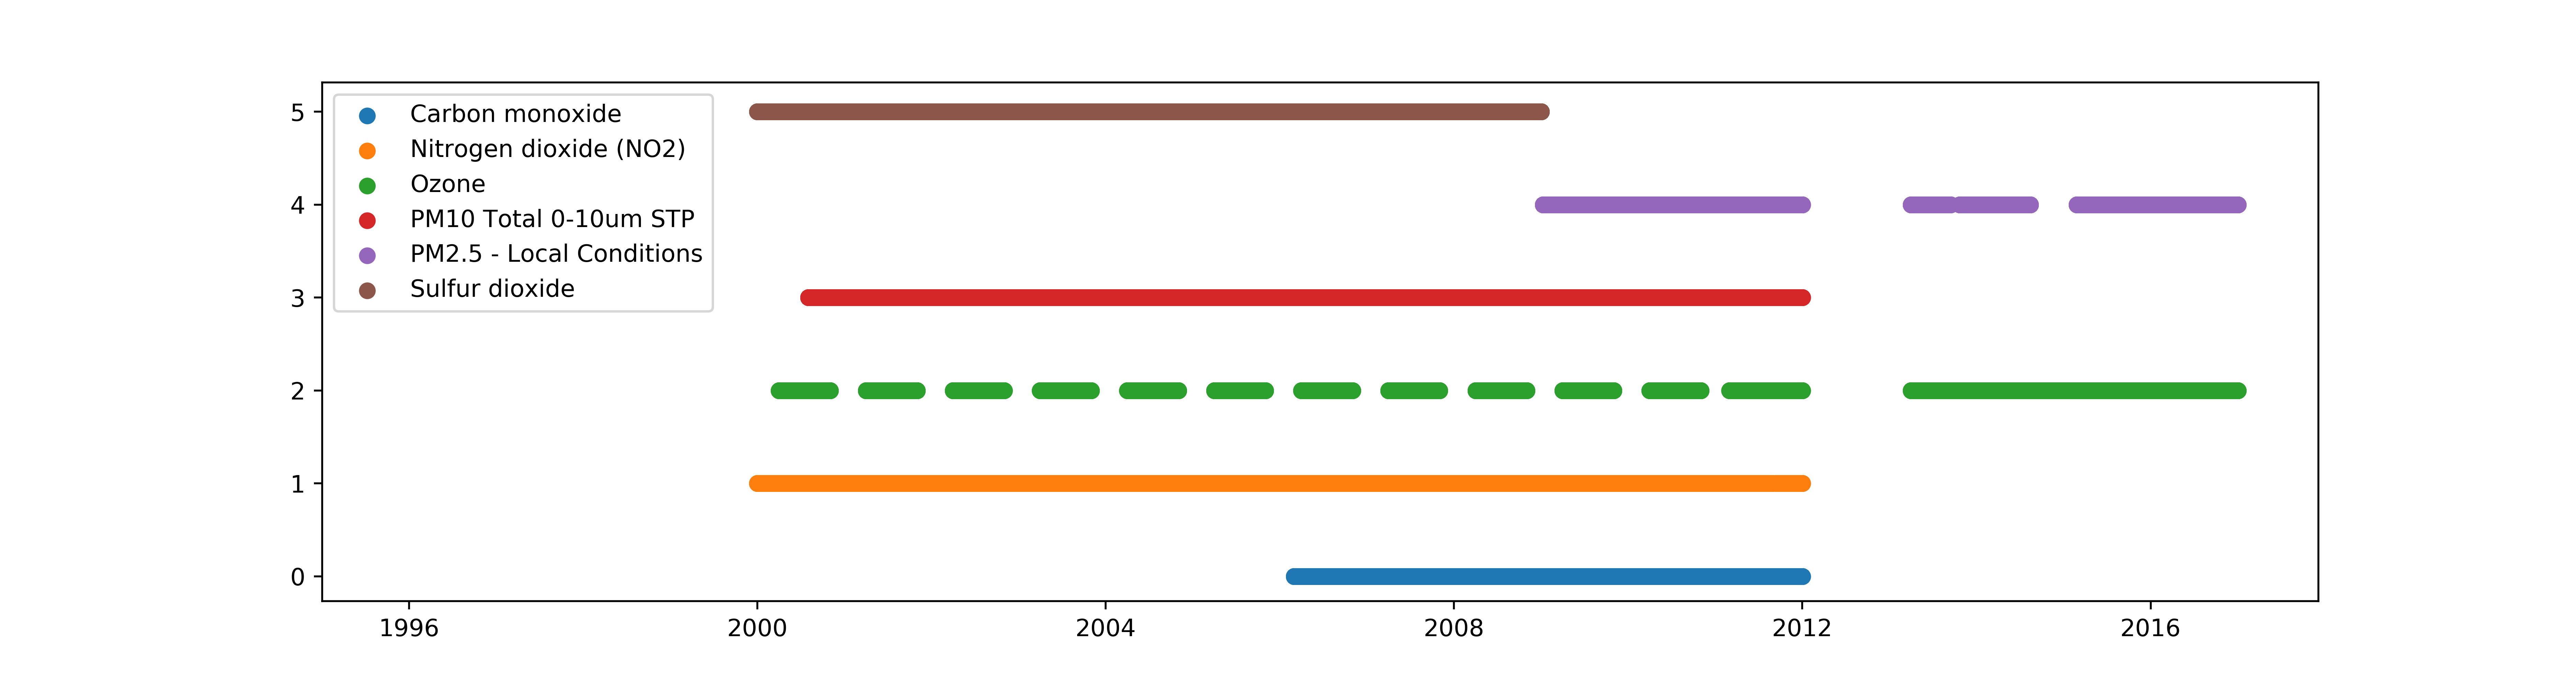
\includegraphics[width=3in]{figs/data_availability}
% \caption{Availability of measurement data for various pollutants}
% \label{data_availability}
% \end{figure}



% if have a single appendix:
%\appendix[Proof of the Zonklar Equations]
% or
%\appendix  % for no appendix heading
% do not use \section anymore after \appendix, only \section*
% is possibly needed

% use appendices with more than one appendix
% then use \section to start each appendix
% you must declare a \section before using any
% \subsection or using \label (\appendices by itself
% starts a section numbered zero.)
%


% \appendices
% \section{Proof of the First Zonklar Equation}
% Some text for the appendix.

% use section* for acknowledgement
% \section*{Acknowledgment}


% The authors would like to thank...


% Can use something like this to put references on a page
% by themselves when using endfloat and the captionsoff option.
\ifCLASSOPTIONcaptionsoff
  \newpage
\fi

\newpage

% trigger a \newpage just before the given reference
% number - used to balance the columns on the last page
% adjust value as needed - may need to be readjusted if
% the document is modified later
\IEEEtriggeratref{6}
% The "triggered" command can be changed if desired:
%\IEEEtriggercmd{\enlargethispage{-5in}}

% references section

% can use a bibliography generated by BibTeX as a .bbl file
% BibTeX documentation can be easily obtained at:
% http://www.ctan.org/tex-archive/biblio/bibtex/contrib/doc/
% The IEEEtran BibTeX style support page is at:
% http://www.michaelshell.org/tex/ieeetran/bibtex/
\bibliographystyle{IEEEtran}
% argument is your BibTeX string definitions and bibliography database(s)
\bibliography{bib.bib}
% IEEEabrv, 
%
% <OR> manually copy in the resultant .bbl file
% set second argument of \begin to the number of references
% (used to reserve space for the reference number labels box)
% \begin{thebibliography}{1}

% \bibitem{IEEEhowto:kopka}
% H.~Kopka and P.~W. Daly, \emph{A Guide to \LaTeX}, 3rd~ed.\hskip 1em plus
%   0.5em minus 0.4em\relax Harlow, England: Addison-Wesley, 1999.


% \bibitem{IEEEhowto:kopka}
% TODO

% http://www.tandfonline.com/doi/abs/10.1080/10473289.2006.10464485


% http://science.sciencemag.org/content/308/5723/804.full


% http://www.atsjournals.org/doi/abs/10.1164/rccm.200403-333OC


% https://www.weather.gov/ctp/climateNormalsHarrisburg


% Eggert, Gerald G., Harrisburg Industrializes: The Coming of Factories to an American Community. University Park, PA: The Pennsylvania State University Press, 1993.


% http://www.isaet.org/images/extraimages/P513673.pdf 
  
% \end{thebibliography}

% biography section
% 
% If you have an EPS/PDF photo (graphicx package needed) extra braces are
% needed around the contents of the optional argument to biography to prevent
% the LaTeX parser from getting confused when it sees the complicated
% \includegraphics command within an optional argument. (You could create
% your own custom macro containing the \includegraphics command to make things
% simpler here.)
%\begin{biography}[{\includegraphics[width=1in,height=1.25in,clip,keepaspectratio]{mshell}}]{Michael Shell}
% or if you just want to reserve a space for a photo:

% \begin{IEEEbiography}[{\includegraphics[width=1in,height=1.25in,clip,keepaspectratio]{picture}}]{John Doe}
% \blindtext
% \end{IEEEbiography}

% You can push biographies down or up by placing
% a \vfill before or after them. The appropriate
% use of \vfill depends on what kind of text is
% on the last page and whether or not the columns
% are being equalized.

%\vfill

% Can be used to pull up biographies so that the bottom of the last one
% is flush with the other column.
%\enlargethispage{-5in}



% \begin{tabular}{ l c r }
%   1 & 2 & 3 \\
%   4 & 5 & 6 \\
%   7 & 8 & 9 \\
% \end{tabular}




% that's all folks
\end{document}


% An example of a double column floating figure using two subfigures.
% (The subfig.sty package must be loaded for this to work.)
% The subfigure \label commands are set within each subfloat command, the
% \label for the overall figure must come after \caption.
% \hfil must be used as a separator to get equal spacing.
% The subfigure.sty package works much the same way, except \subfigure is
% used instead of \subfloat.
%
%\begin{figure*}[!t]
%\centerline{\subfloat[Case I]\includegraphics[width=2.5in]{subfigcase1}%
%\label{fig_first_case}}
%\hfil
%\subfloat[Case II]{\includegraphics[width=2.5in]{subfigcase2}%
%\label{fig_second_case}}}
%\caption{Simulation results}
%\label{fig_sim}
%\end{figure*}
%
% Note that often IEEE papers with subfigures do not employ subfigure
% captions (using the optional argument to \subfloat), but instead will
% reference/describe all of them (a), (b), etc., within the main caption.


% An example of a floating table. Note that, for IEEE style tables, the 
% \caption command should come BEFORE the table. Table text will default to
% \footnotesize as IEEE normally uses this smaller font for tables.
% The \label must come after \caption as always.
%
%\begin{table}[!t]
%% increase table row spacing, adjust to taste
%\renewcommand{\arraystretch}{1.3}
% if using array.sty, it might be a good idea to tweak the value of
% \extrarowheight as needed to properly center the text within the cells
%\caption{An Example of a Table}
%\label{table_example}
%\centering
%% Some packages, such as MDW tools, offer better commands for making tables
%% than the plain LaTeX2e tabular which is used here.
%\begin{tabular}{|c||c|}
%\hline
%One & Two\\
%\hline
%Three & Four\\
%\hline
%\end{tabular}
%\end{table}

% Note that IEEE does not put floats in the very first column - or typically
% anywhere on the first page for that matter. Also, in-text middle ("here")
% positioning is not used. Most IEEE journals use top floats exclusively.
% Note that, LaTeX2e, unlike IEEE journals, places footnotes above bottom
% floats. This can be corrected via the \fnbelowfloat command of the
% stfloats package.
